% Options for packages loaded elsewhere
\PassOptionsToPackage{unicode}{hyperref}
\PassOptionsToPackage{hyphens}{url}
%
\documentclass[
]{article}
\usepackage{amsmath,amssymb}
\usepackage{lmodern}
\usepackage{ifxetex,ifluatex}
\ifnum 0\ifxetex 1\fi\ifluatex 1\fi=0 % if pdftex
  \usepackage[T1]{fontenc}
  \usepackage[utf8]{inputenc}
  \usepackage{textcomp} % provide euro and other symbols
\else % if luatex or xetex
  \usepackage{unicode-math}
  \defaultfontfeatures{Scale=MatchLowercase}
  \defaultfontfeatures[\rmfamily]{Ligatures=TeX,Scale=1}
\fi
% Use upquote if available, for straight quotes in verbatim environments
\IfFileExists{upquote.sty}{\usepackage{upquote}}{}
\IfFileExists{microtype.sty}{% use microtype if available
  \usepackage[]{microtype}
  \UseMicrotypeSet[protrusion]{basicmath} % disable protrusion for tt fonts
}{}
\makeatletter
\@ifundefined{KOMAClassName}{% if non-KOMA class
  \IfFileExists{parskip.sty}{%
    \usepackage{parskip}
  }{% else
    \setlength{\parindent}{0pt}
    \setlength{\parskip}{6pt plus 2pt minus 1pt}}
}{% if KOMA class
  \KOMAoptions{parskip=half}}
\makeatother
\usepackage{xcolor}
\IfFileExists{xurl.sty}{\usepackage{xurl}}{} % add URL line breaks if available
\IfFileExists{bookmark.sty}{\usepackage{bookmark}}{\usepackage{hyperref}}
\hypersetup{
  pdftitle={Mapping scientific communities at scale},
  pdfkeywords={French publications, IPCC, IPBES, Machine
learning, NLP, open data, open source, scanR, OpenAlex},
  hidelinks,
  pdfcreator={LaTeX via pandoc}}
\urlstyle{same} % disable monospaced font for URLs
\usepackage[left=3cm, right=3cm, top=3cm, bottom=3cm]{geometry}
\usepackage{color}
\usepackage{fancyvrb}
\newcommand{\VerbBar}{|}
\newcommand{\VERB}{\Verb[commandchars=\\\{\}]}
\DefineVerbatimEnvironment{Highlighting}{Verbatim}{commandchars=\\\{\}}
% Add ',fontsize=\small' for more characters per line
\newenvironment{Shaded}{}{}
\newcommand{\AlertTok}[1]{\textcolor[rgb]{1.00,0.00,0.00}{\textbf{#1}}}
\newcommand{\AnnotationTok}[1]{\textcolor[rgb]{0.38,0.63,0.69}{\textbf{\textit{#1}}}}
\newcommand{\AttributeTok}[1]{\textcolor[rgb]{0.49,0.56,0.16}{#1}}
\newcommand{\BaseNTok}[1]{\textcolor[rgb]{0.25,0.63,0.44}{#1}}
\newcommand{\BuiltInTok}[1]{#1}
\newcommand{\CharTok}[1]{\textcolor[rgb]{0.25,0.44,0.63}{#1}}
\newcommand{\CommentTok}[1]{\textcolor[rgb]{0.38,0.63,0.69}{\textit{#1}}}
\newcommand{\CommentVarTok}[1]{\textcolor[rgb]{0.38,0.63,0.69}{\textbf{\textit{#1}}}}
\newcommand{\ConstantTok}[1]{\textcolor[rgb]{0.53,0.00,0.00}{#1}}
\newcommand{\ControlFlowTok}[1]{\textcolor[rgb]{0.00,0.44,0.13}{\textbf{#1}}}
\newcommand{\DataTypeTok}[1]{\textcolor[rgb]{0.56,0.13,0.00}{#1}}
\newcommand{\DecValTok}[1]{\textcolor[rgb]{0.25,0.63,0.44}{#1}}
\newcommand{\DocumentationTok}[1]{\textcolor[rgb]{0.73,0.13,0.13}{\textit{#1}}}
\newcommand{\ErrorTok}[1]{\textcolor[rgb]{1.00,0.00,0.00}{\textbf{#1}}}
\newcommand{\ExtensionTok}[1]{#1}
\newcommand{\FloatTok}[1]{\textcolor[rgb]{0.25,0.63,0.44}{#1}}
\newcommand{\FunctionTok}[1]{\textcolor[rgb]{0.02,0.16,0.49}{#1}}
\newcommand{\ImportTok}[1]{#1}
\newcommand{\InformationTok}[1]{\textcolor[rgb]{0.38,0.63,0.69}{\textbf{\textit{#1}}}}
\newcommand{\KeywordTok}[1]{\textcolor[rgb]{0.00,0.44,0.13}{\textbf{#1}}}
\newcommand{\NormalTok}[1]{#1}
\newcommand{\OperatorTok}[1]{\textcolor[rgb]{0.40,0.40,0.40}{#1}}
\newcommand{\OtherTok}[1]{\textcolor[rgb]{0.00,0.44,0.13}{#1}}
\newcommand{\PreprocessorTok}[1]{\textcolor[rgb]{0.74,0.48,0.00}{#1}}
\newcommand{\RegionMarkerTok}[1]{#1}
\newcommand{\SpecialCharTok}[1]{\textcolor[rgb]{0.25,0.44,0.63}{#1}}
\newcommand{\SpecialStringTok}[1]{\textcolor[rgb]{0.73,0.40,0.53}{#1}}
\newcommand{\StringTok}[1]{\textcolor[rgb]{0.25,0.44,0.63}{#1}}
\newcommand{\VariableTok}[1]{\textcolor[rgb]{0.10,0.09,0.49}{#1}}
\newcommand{\VerbatimStringTok}[1]{\textcolor[rgb]{0.25,0.44,0.63}{#1}}
\newcommand{\WarningTok}[1]{\textcolor[rgb]{0.38,0.63,0.69}{\textbf{\textit{#1}}}}
\usepackage{graphicx}
\makeatletter
\def\maxwidth{\ifdim\Gin@nat@width>\linewidth\linewidth\else\Gin@nat@width\fi}
\def\maxheight{\ifdim\Gin@nat@height>\textheight\textheight\else\Gin@nat@height\fi}
\makeatother
% Scale images if necessary, so that they will not overflow the page
% margins by default, and it is still possible to overwrite the defaults
% using explicit options in \includegraphics[width, height, ...]{}
\setkeys{Gin}{width=\maxwidth,height=\maxheight,keepaspectratio}
% Set default figure placement to htbp
\makeatletter
\def\fps@figure{htbp}
\makeatother
\setlength{\emergencystretch}{3em} % prevent overfull lines
\providecommand{\tightlist}{%
  \setlength{\itemsep}{0pt}\setlength{\parskip}{0pt}}
\setcounter{secnumdepth}{-\maxdimen} % remove section numbering
\ifluatex
  \usepackage{selnolig}  % disable illegal ligatures
\fi
\newlength{\cslhangindent}
\setlength{\cslhangindent}{1.5em}
\newlength{\csllabelwidth}
\setlength{\csllabelwidth}{3em}
\newenvironment{CSLReferences}[2] % #1 hanging-ident, #2 entry spacing
 {% don't indent paragraphs
  \setlength{\parindent}{0pt}
  % turn on hanging indent if param 1 is 1
  \ifodd #1 \everypar{\setlength{\hangindent}{\cslhangindent}}\ignorespaces\fi
  % set entry spacing
  \ifnum #2 > 0
  \setlength{\parskip}{#2\baselineskip}
  \fi
 }%
 {}
\usepackage{calc}
\newcommand{\CSLBlock}[1]{#1\hfill\break}
\newcommand{\CSLLeftMargin}[1]{\parbox[t]{\csllabelwidth}{#1}}
\newcommand{\CSLRightInline}[1]{\parbox[t]{\linewidth - \csllabelwidth}{#1}\break}
\newcommand{\CSLIndent}[1]{\hspace{\cslhangindent}#1}
% for compatibility with pandoc 2.10
\newenvironment{cslreferences}%
  {\setlength{\parindent}{0pt}%
  \everypar{\setlength{\hangindent}{\cslhangindent}}\ignorespaces}%
  {\par}

\title{Mapping scientific communities at scale}
\usepackage{authblk}
\author[%
  1%
  ]{%
  Hafsa Aallat%
  %
  %
}
\affil[1]{French Ministry of Higher Education and Research, Paris,
France}
\date{February 2025}

\makeatletter
\def\@maketitle{%
  \newpage \null \vskip 2em
  \begin {center}%
    \let \footnote \thanks
         {\LARGE \@title \par}%
         \vskip 1.5em%
                {\large \lineskip .5em%
                  \begin {tabular}[t]{c}%
                    \@author
                  \end {tabular}\par}%
                                                \vskip 1em{\large \@date}%
  \end {center}%
  \par
  \vskip 1.5em}
\makeatother

\begin{document}
\maketitle

\textbf{Keywords}: French publications, IPCC, IPBES, Machine learning,
NLP, open data, open source, scanR, OpenAlex

\hypertarget{motivation}{%
\section{1. Motivation}\label{motivation}}

\hypertarget{presentation-of-ipcc-and-ipbes-working-groups-and-dates}{%
\subsection{1.1 Presentation of IPCC and IPBES: Working Groups and
dates}\label{presentation-of-ipcc-and-ipbes-working-groups-and-dates}}

\textbf{The IPCC (Intergovernmental Panel on Climate Change)} assesses
scientific information on climate change, providing reports to guide
policymakers. It has three working groups sees as three main topics :

\begin{itemize}
\tightlist
\item
  Working Group 1 (WG1) focuses on the \textbf{physical science} of
  climate change.
\item
  Working Group 2 (WG2) examines climate change impacts,
  \textbf{adaptation}, and vulnerabilities.
\item
  Working Group 2 - cross chapters (WG2 cross) addresses the
  interactions between physical science and impacts, adaptation, and
  vulnerabilities.
\item
  Working Group 3 (WG3) addresses climate change \textbf{mitigation}
  strategies.
\end{itemize}

The Sixth Assessment Report (AR6) was released in stages between 2021
and 2022.

\textbf{The IPBES (Intergovernmental Science-Policy Platform on
Biodiversity and Ecosystem Services)}, established in 2012, assesses
biodiversity and ecosystem services. It produces thematic and regional
assessments, with the \textbf{Global Assessment Report (2019)}
highlighting biodiversity loss and the need for urgent action.

Both platforms provide crucial scientific assessments that inform global
climate and biodiversity policies.

\hypertarget{limits-of-the-french-court-of-audit-study}{%
\subsection{1.2 Limits of the French Court of Audit
study}\label{limits-of-the-french-court-of-audit-study}}

In 2023, the French Court of Audit conducted a study on France's
scientific output related to environmental transition. After hearings
with the Directorate General for Research and Innovation (DGRI) and
research operators, the Court analyzed the bibliography cited in the
sixth IPCC report. The study found that French publications are the most
cited in the physical sciences of climate change, highlighting the
global impact of French research in this field.

However, this evaluation has important limitations. The IPCC
bibliography is based on high-impact publications often from top
journals, making it quite selective. This selection prioritizes more
visible and well-known works, leaving out other important research that
may not be as visible but still in the same topics as IPCC report. While
this reflects France's scientific excellence, it does not fully
represent the diversity of French scientific contributions to ecological
transition.

\hypertarget{how-can-we-explore-and-recognize-french-publications-related-to-the-same-topics-as-ipcc-and-ipbes-report-from-a-larger-point-of-view}{%
\subsection{1.3 How can we explore and recognize french publications
related to the same topics as IPCC and IPBES report from a larger point
of view
?}\label{how-can-we-explore-and-recognize-french-publications-related-to-the-same-topics-as-ipcc-and-ipbes-report-from-a-larger-point-of-view}}

To fill this gap, we propose using a larger dataset, such as scanR.
\textbf{ScanR has a significantly higher coverage} of publications with
at least one French affiliation compared to other sources, contributing
92\% to the overall aggregated corpus. This is much higher than
databases like Scopus (67\%), WoS (58\%), or PubMed (29\%), making ScanR
a more comprehensive tool for capturing French scientific publications
(Chaignon and Egret 2022). Unlike the IPCC's restricted approach, ScanR
includes publications with at least one French affiliation, showing a
larger view of research. This could allow us to capture a more diverse
range of topics related to climate change physical science, adaptation
and mitigation.

Initially, we will replicate the Court of Audit analysis of the IPCC
bibliography to identify the main topics and their proportion of French
contributions. Then, we will expand our study to know the top
institutions, labs, regions, and researchers that provide solutions to
the challenges of environemental transition in France, based on IPCC
bibliography. In a second time, we will create a model that can
recognize a publication about IPCC similar topics, and apply the model
to scanR publications. At the same time, we will conduct a similar
analysis for the IPBES bibliography, following the same approach to
identify the French contributions, and exploring less visible but
valuable research related to biodiversity and ecosystem services.

\hypertarget{ipcc-and-ipbes-bibliography-analysis-and-model}{%
\section{2. IPCC and IPBES Bibliography Analysis and
Model}\label{ipcc-and-ipbes-bibliography-analysis-and-model}}

We propose a method to analyze the bibliographies of IPCC and IPBES
reports.

\hypertarget{data-collection-and-cleaning}{%
\subsection{2.1 Data Collection and
Cleaning}\label{data-collection-and-cleaning}}

For each report, we collect the references:

\begin{itemize}
\tightlist
\item
  For IPCC report, we collect citations in .bib format for each chapter
  of each working group (n.d.a).
\item
  For IPBES report, we gather all citations via Zotero (n.d.b).
\end{itemize}

Once the data is collected, we clean the DOI (Digital Object Identifier)
of each publication. The DOI should follow a specific format starting
with `10.'. Any publication without a valid DOI is not considered.

\hypertarget{data-enrichment}{%
\subsection{2.2 Data Enrichment}\label{data-enrichment}}

After cleaning, the data contains features such as DOI, title, and main
author. However, we still lack information such as institutions,
researchers, countries, and topics associated with each publication. To
fill in the gap, we enrich the data by importing additional features
from OpenAlex for each publication with a valid DOI. These features
include: countries, year, topics, title, author names, institutions,
RORs (Research Organization Registry) and journals.

OpenAlex is an international open-access database that provides metadata
on research papers, authors, journals, and institutions. It aims to make
academic information more accessible and supports data analysis and
knowledge discovery in various fields. OpenAlex is a valuable tool for
researchers and educators. We use the Api to import the features.

Next, we use the Biblioglutton Python library to fill in missing DOIs
based on the title and main author. We also verify that the year
retrieved from OpenAlex matches the year in the original dataset.

\hypertarget{data-storage-and-visualization}{%
\subsection{2.3 Data storage and
visualization}\label{data-storage-and-visualization}}

Once the data is enriched with openAlex features, we edit the data and
push them on a cluster elastic-search. As an exemple, for one
publication (for a better visibility the data is troncated). Some
publications are used by both reports, with the following keys:

\begin{Shaded}
\begin{Highlighting}[]
\FunctionTok{\{}
  \DataTypeTok{"doi"}\FunctionTok{:} \StringTok{"10.1126/science.aaw6974"}\FunctionTok{,}
  \DataTypeTok{"year"}\FunctionTok{:} \StringTok{"2018"}\FunctionTok{,}
  \DataTypeTok{"title"}\FunctionTok{:} \StringTok{"Impacts of 1.5 °C global warming on natural and human systems"}\FunctionTok{,}
  \DataTypeTok{"rors"}\FunctionTok{:} \OtherTok{[}
    \OtherTok{[}\StringTok{"https://ror.org/00rqy9422"}\OtherTok{,} \StringTok{"AU"}\OtherTok{],}
    \OtherTok{[}\StringTok{"https://ror.org/03ztgj037"}\OtherTok{,} \StringTok{"DE"}\OtherTok{],}
    \OtherTok{[}\StringTok{"https://ror.org/05sbt2524"}\OtherTok{,} \StringTok{"FR"}\OtherTok{],}
    \OtherTok{[}\StringTok{"..."}\OtherTok{]}
  \OtherTok{]}\FunctionTok{,}
  \DataTypeTok{"ipcc"}\FunctionTok{:} \OtherTok{[}
    \FunctionTok{\{} \DataTypeTok{"name"}\FunctionTok{:} \StringTok{"wg1\_chap\_01"}\FunctionTok{,} \DataTypeTok{"wg"}\FunctionTok{:} \StringTok{"1"}\FunctionTok{,} \DataTypeTok{"chap"}\FunctionTok{:} \DecValTok{1} \FunctionTok{\}}\OtherTok{,}
    \FunctionTok{\{} \DataTypeTok{"name"}\FunctionTok{:} \StringTok{"wg2\_chap\_01"}\FunctionTok{,} \DataTypeTok{"wg"}\FunctionTok{:} \StringTok{"2"}\FunctionTok{,} \DataTypeTok{"chap"}\FunctionTok{:} \DecValTok{1} \FunctionTok{\}}\OtherTok{,}
    \FunctionTok{\{} \DataTypeTok{"name"}\FunctionTok{:} \StringTok{"wg2\_chap\_02"}\FunctionTok{,} \DataTypeTok{"wg"}\FunctionTok{:} \StringTok{"2"}\FunctionTok{,} \DataTypeTok{"chap"}\FunctionTok{:} \DecValTok{2} \FunctionTok{\}}\OtherTok{,}
    \FunctionTok{\{} \DataTypeTok{"name"}\FunctionTok{:} \StringTok{"wg2\_chap\_04"}\FunctionTok{,} \DataTypeTok{"wg"}\FunctionTok{:} \StringTok{"2"}\FunctionTok{,} \DataTypeTok{"chap"}\FunctionTok{:} \DecValTok{4} \FunctionTok{\}}\OtherTok{,}
    \FunctionTok{\{} \DataTypeTok{"name"}\FunctionTok{:} \StringTok{"wg2\_chap\_07"}\FunctionTok{,} \DataTypeTok{"wg"}\FunctionTok{:} \StringTok{"2"}\FunctionTok{,} \DataTypeTok{"chap"}\FunctionTok{:} \DecValTok{7} \FunctionTok{\}}\OtherTok{,}
    \FunctionTok{\{} \DataTypeTok{"name"}\FunctionTok{:} \StringTok{"wg2\_chap\_08"}\FunctionTok{,} \DataTypeTok{"wg"}\FunctionTok{:} \StringTok{"2"}\FunctionTok{,} \DataTypeTok{"chap"}\FunctionTok{:} \DecValTok{8} \FunctionTok{\}}\OtherTok{,}
    \FunctionTok{\{} \DataTypeTok{"name"}\FunctionTok{:} \StringTok{"wg2\_chap\_12"}\FunctionTok{,} \DataTypeTok{"wg"}\FunctionTok{:} \StringTok{"2"}\FunctionTok{,} \DataTypeTok{"chap"}\FunctionTok{:} \DecValTok{12} \FunctionTok{\}}\OtherTok{,}
    \FunctionTok{\{} \DataTypeTok{"name"}\FunctionTok{:} \StringTok{"wg2\_chap\_13"}\FunctionTok{,} \DataTypeTok{"wg"}\FunctionTok{:} \StringTok{"2"}\FunctionTok{,} \DataTypeTok{"chap"}\FunctionTok{:} \DecValTok{13} \FunctionTok{\}}\OtherTok{,}
    \FunctionTok{\{} \DataTypeTok{"name"}\FunctionTok{:} \StringTok{"wg2\_chap\_14"}\FunctionTok{,} \DataTypeTok{"wg"}\FunctionTok{:} \StringTok{"2"}\FunctionTok{,} \DataTypeTok{"chap"}\FunctionTok{:} \DecValTok{14} \FunctionTok{\}}\OtherTok{,}
    \FunctionTok{\{} \DataTypeTok{"name"}\FunctionTok{:} \StringTok{"wg2\_chap\_15"}\FunctionTok{,} \DataTypeTok{"wg"}\FunctionTok{:} \StringTok{"2"}\FunctionTok{,} \DataTypeTok{"chap"}\FunctionTok{:} \DecValTok{15} \FunctionTok{\}}\OtherTok{,}
    \FunctionTok{\{} \DataTypeTok{"name"}\FunctionTok{:} \StringTok{"wg2\_chap\_16"}\FunctionTok{,} \DataTypeTok{"wg"}\FunctionTok{:} \StringTok{"2"}\FunctionTok{,} \DataTypeTok{"chap"}\FunctionTok{:} \DecValTok{16} \FunctionTok{\}}\OtherTok{,}
    \FunctionTok{\{} \DataTypeTok{"name"}\FunctionTok{:} \StringTok{"wg2\_cross\_chap\_1"}\FunctionTok{,} \DataTypeTok{"wg"}\FunctionTok{:} \StringTok{"2\_cross"}\FunctionTok{,} \DataTypeTok{"chap"}\FunctionTok{:} \DecValTok{1} \FunctionTok{\}}\OtherTok{,}
    \FunctionTok{\{} \DataTypeTok{"name"}\FunctionTok{:} \StringTok{"wg2\_cross\_chap\_4"}\FunctionTok{,} \DataTypeTok{"wg"}\FunctionTok{:} \StringTok{"2\_cross"}\FunctionTok{,} \DataTypeTok{"chap"}\FunctionTok{:} \DecValTok{4} \FunctionTok{\}}\OtherTok{,}
    \FunctionTok{\{} \DataTypeTok{"name"}\FunctionTok{:} \StringTok{"wg3\_chap\_01"}\FunctionTok{,} \DataTypeTok{"wg"}\FunctionTok{:} \StringTok{"3"}\FunctionTok{,} \DataTypeTok{"chap"}\FunctionTok{:} \DecValTok{1} \FunctionTok{\}}\OtherTok{,}
    \FunctionTok{\{} \DataTypeTok{"name"}\FunctionTok{:} \StringTok{"wg3\_chap\_04"}\FunctionTok{,} \DataTypeTok{"wg"}\FunctionTok{:} \StringTok{"3"}\FunctionTok{,} \DataTypeTok{"chap"}\FunctionTok{:} \DecValTok{4} \FunctionTok{\}}
  \OtherTok{]}\FunctionTok{,}
  \DataTypeTok{"authors\_name"}\FunctionTok{:} \OtherTok{[}
    \OtherTok{[}\StringTok{"Ove Hoegh‐Guldberg"}\OtherTok{,} \OtherTok{[}\StringTok{"AU"}\OtherTok{]],}
    \OtherTok{[}\StringTok{"Daniela Jacob"}\OtherTok{,} \OtherTok{[}\StringTok{"DE"}\OtherTok{]],}
    \OtherTok{[}\StringTok{"Michael A. Taylor"}\OtherTok{,} \OtherTok{[}\StringTok{"JM"}\OtherTok{]],}
    \OtherTok{[}\StringTok{"..."}\OtherTok{]}
  \OtherTok{]}\FunctionTok{,}
  \DataTypeTok{"institutions\_names"}\FunctionTok{:} \OtherTok{[}
    \OtherTok{[}\StringTok{"University of Queensland"}\OtherTok{,} \StringTok{"AU"}\OtherTok{],}
    \OtherTok{[}\StringTok{"German Climate Computing Centre"}\OtherTok{,} \StringTok{"DE"}\OtherTok{],}
    \OtherTok{[}\StringTok{"University of the West Indies"}\OtherTok{,} \StringTok{"JM"}\OtherTok{],}
    \OtherTok{[}\StringTok{"..."}\OtherTok{]}
  \OtherTok{]}\FunctionTok{,}
  \DataTypeTok{"countries"}\FunctionTok{:} \OtherTok{[}\StringTok{"CHN"}\OtherTok{,} \StringTok{"GBR"}\OtherTok{,} \StringTok{"FRA"}\OtherTok{,} \StringTok{"..."}\OtherTok{]}\FunctionTok{,}
  \DataTypeTok{"ipbes"}\FunctionTok{:} \OtherTok{[}\FunctionTok{\{} \DataTypeTok{"chapter"}\FunctionTok{:} \StringTok{"4"} \FunctionTok{\}}\OtherTok{]}\FunctionTok{,}
  \DataTypeTok{"topics"}\FunctionTok{:} \OtherTok{[}
    \StringTok{"Impact of Climate Change on Human Migration"}\OtherTok{,}
    \StringTok{"Geoengineering and Climate Ethics"}\OtherTok{,}
    \StringTok{"Economic Implications of Climate Change Policies"}
  \OtherTok{]}
\FunctionTok{\}}
\end{Highlighting}
\end{Shaded}

After that we used Highcharts, a graphic tool to visualize the graphs.
At the same time, we plot the graphs also with python by making
elastic-search requests.

\hypertarget{create-a-database}{%
\subsection{2.4 Create a database}\label{create-a-database}}

In the enriched database from the IPCC and IPBES publications, each
publication is associated with the following attributes:

\begin{itemize}
\tightlist
\item
  A unique identifier (\textbf{DOI})
\item
  The publication \textbf{year}
\item
  A \textbf{title} that best summarizes the publication
\item
  The main \textbf{topics} covered by the publication: publications in
  OpenAlex are tagged with Topics using an automated system that takes
  into account the available information about the work, including
  title, abstract, source (journal) name, and citations
\item
  The names of the \textbf{journals} in which the publication was
  published
\end{itemize}

Out of the 53,258 IPCC publications available on OpenAlex, only 48,219
have non-empty titles, topics, and journal names.

The goal is to identify these 48,219 publications that are not cited by
the IPCC to form our training dataset. After the analysis phase, we were
wondering how to make a database with data from IPCC bibliography and
data from other subjects than IPCC topics.

Initially, we explore the data from the reports and analize:

\begin{itemize}
\tightlist
\item
  Their temporal distribution
\item
  The main topics
\item
  The main journals were the publications are released
\end{itemize}

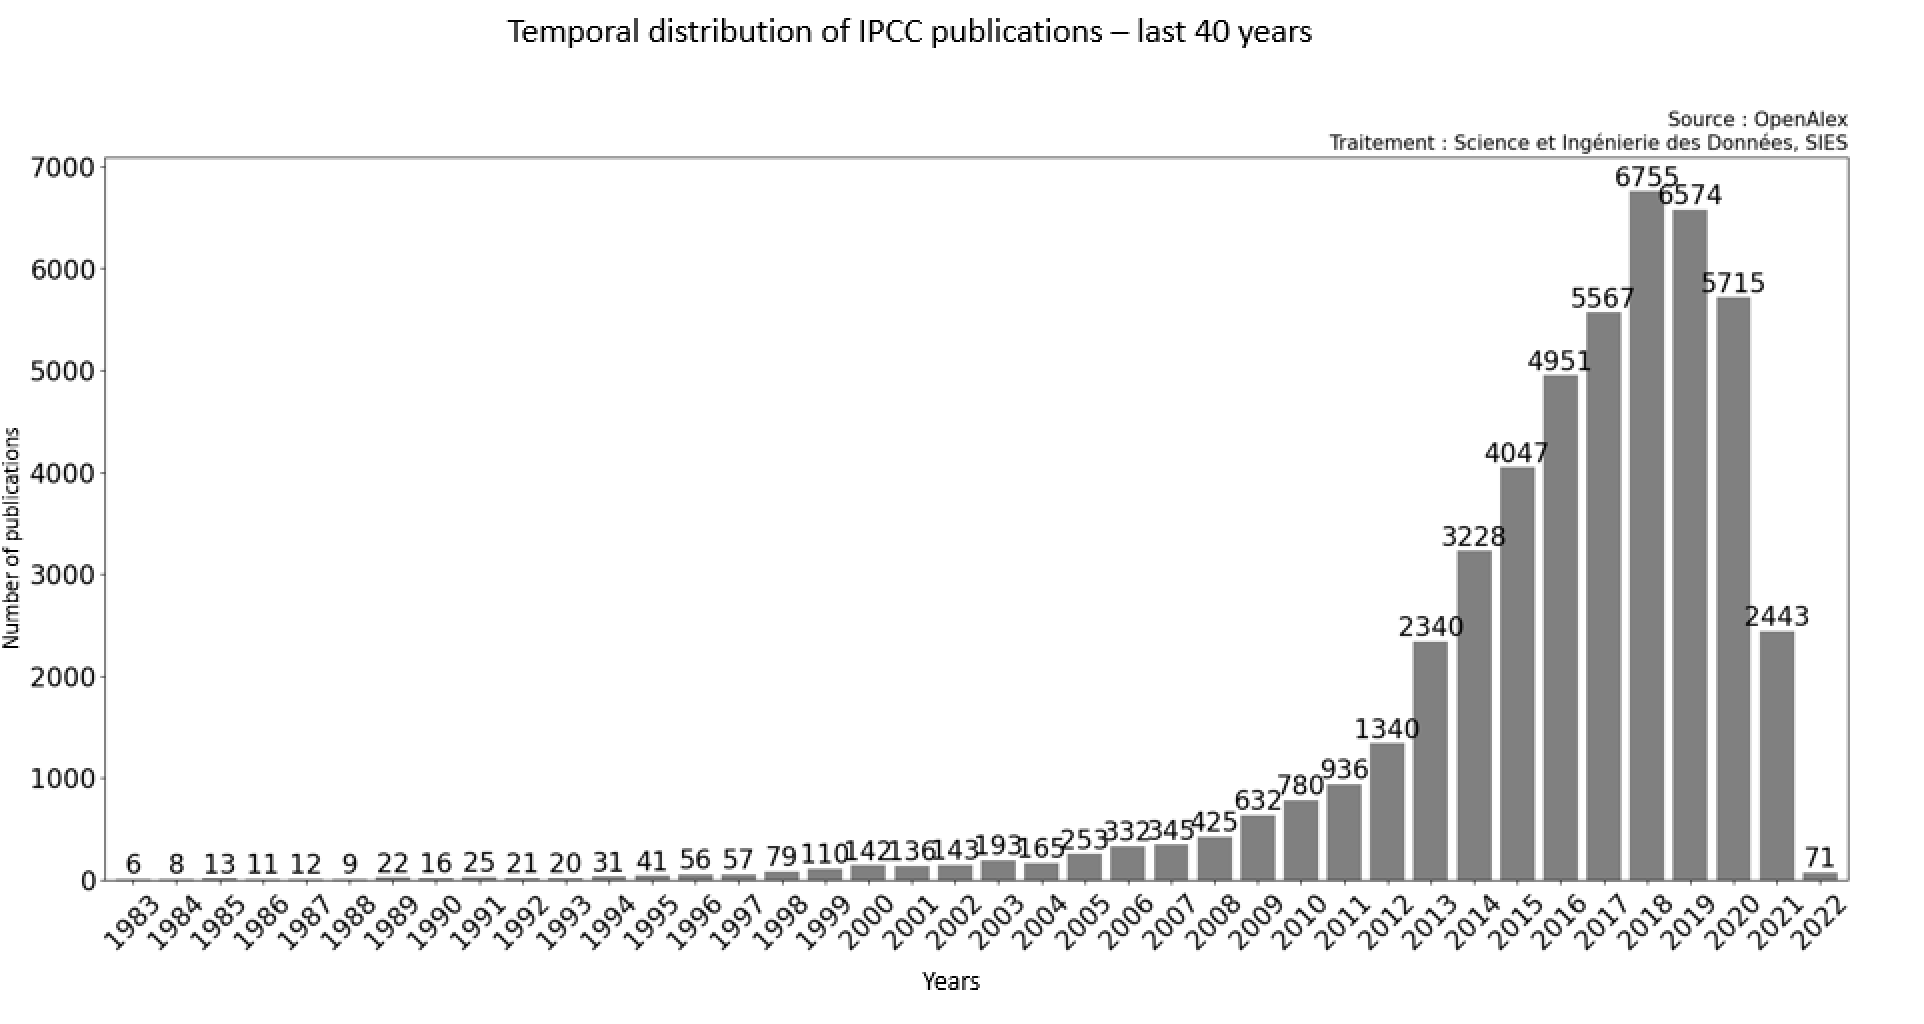
\includegraphics{./images/time_distribution_IPCC_model.png}
\emph{Temporal distribution of French IPCC publications.}

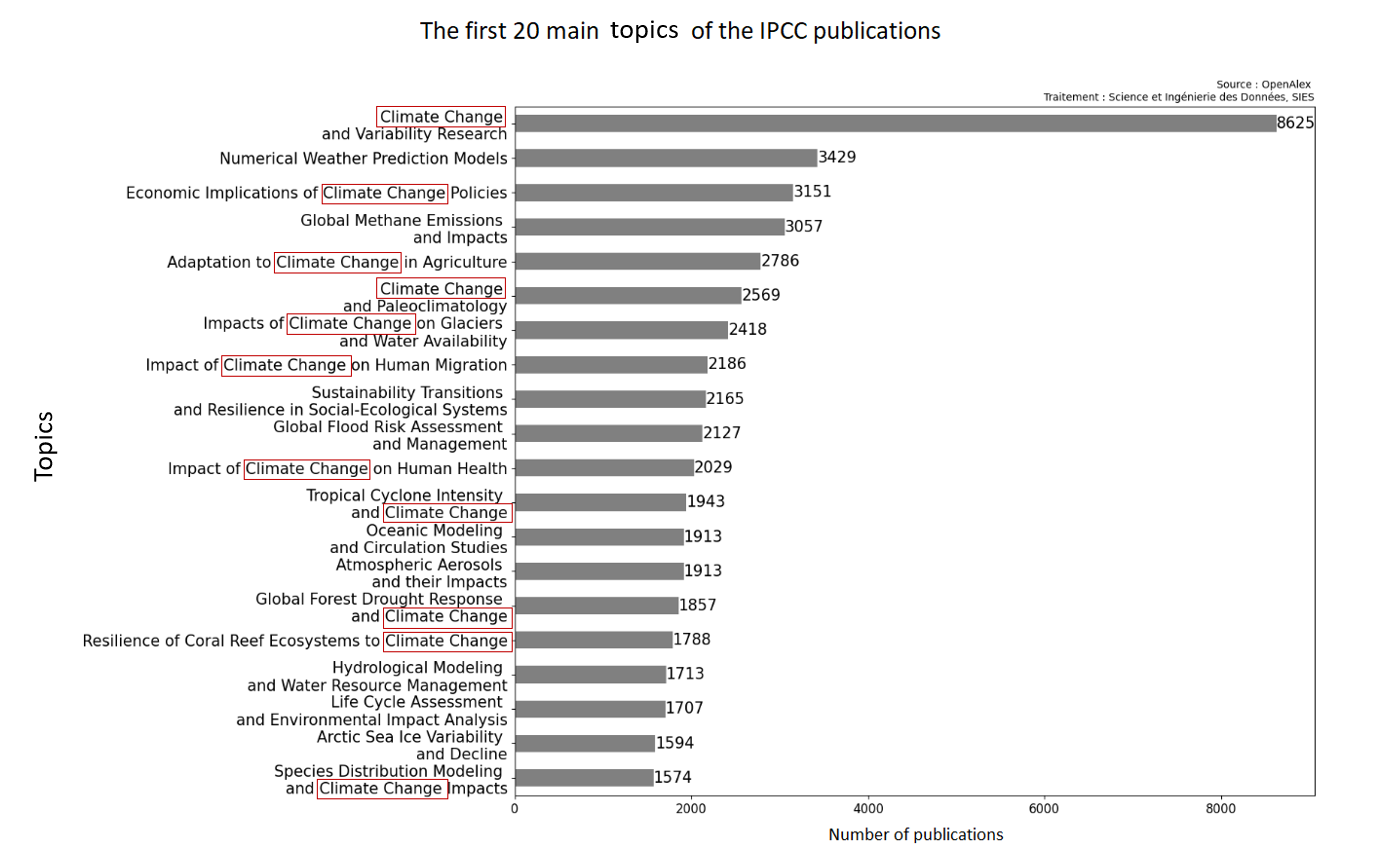
\includegraphics{./images/topics_distribution_IPCC_model.png}
\emph{Topics distribution of French IPCC publications.}

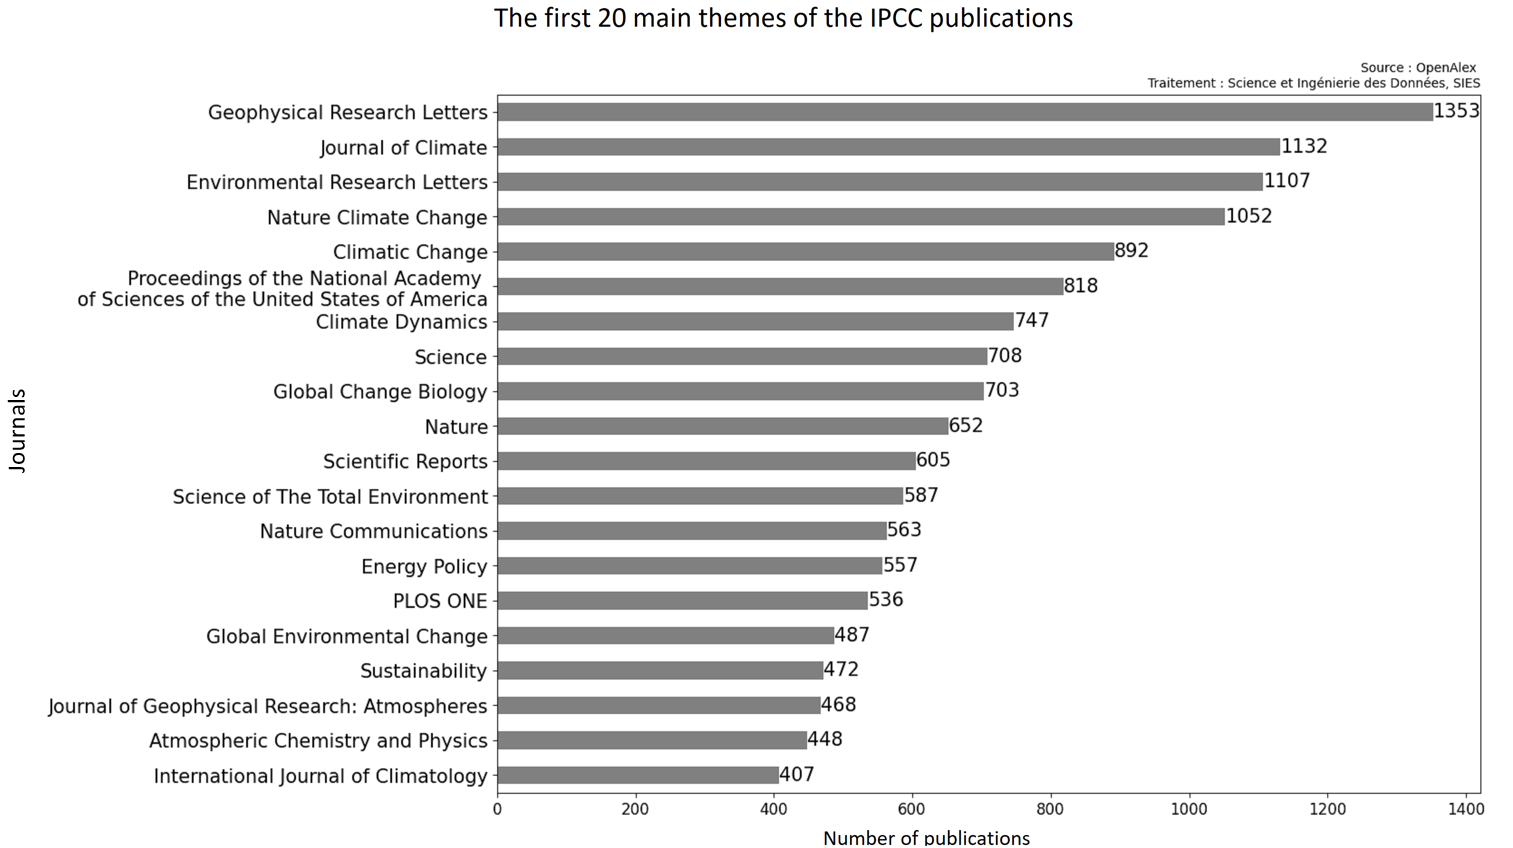
\includegraphics{./images/locations_distribution_IPCC_model.png}
\emph{Journals distribution of French IPCC publications.}

We conclued that the publications from the reports are recents, less
than 10 years old for 90\% of them. Some keywords seems to appear
frequently, like ``Climate Change'' and IPCC publications are mainly
released by scientific journals.

Using the OpenAlex API, we found 48,219 publications that meet the
following criteria:

\begin{enumerate}
\def\labelenumi{\arabic{enumi}.}
\tightlist
\item
  Publications that are \textbf{not cited by the IPCC}.
\item
  Publications that \textbf{do not contain specific terms} according to
  the top topics, such as ``climate change'' or ``environmental impact''
  in their topics, ensuring that our model remains unbiased.
\item
  Publications that have a \textbf{global temporal distribution
  equivalent} to the IPCC's cited publications. For example, in 2018,
  there were 6,755 publications cited by the IPCC, so we retrieve 6,755
  publications from OpenAlex that exclude certain topics. This process
  is repeated for each year in the temporal distribution of IPCC
  publications.
\end{enumerate}

We conduct the exact same method for the IPBES report.

\hypertarget{train-the-model}{%
\subsection{2.5 Train the model}\label{train-the-model}}

Once the dataset is complete, we split it in two:

\begin{itemize}
\tightlist
\item
  80\% of data will be used to train the model
\item
  20\% will be used as a test base
\end{itemize}

To train the model, we use fasttext. FastText is a library developed by
Facebook AI Research for learning word representations and text
classification. Unlike Word2Vec, FastText breaks words into subwords,
improving its ability to handle rare or out-of-vocabulary words. It's
fast, efficient, and supports multilingual models, making it ideal for
various natural language processing tasks like sentiment analysis and
text classification.

Fasttext enable to vectorize and apply a linear regression on the data.
We try 2 kind of model:

\begin{itemize}
\tightlist
\item
  a model that determine if a publication is align with the same topics
  as the IPCC or IPBES report.
\item
  a model to be applied only to ``IPCC-like'' publications, to determine
  the most relevant working group and identify whether the publication
  focuses on physical science, adaptation, or mitigation.
\end{itemize}

\hypertarget{comparative-analysis-of-country-contributions-to-ipcc-reports}{%
\subsection{2.6 Comparative analysis of country contributions to IPCC
Reports}\label{comparative-analysis-of-country-contributions-to-ipcc-reports}}

In the first part of our analysis, we examined the publications from
IPCC reports and compared the contributions of different countries. Now,
we want to evaluate these contributions from a global perspective.

To simplify the process, we apply filters, as using the initial model
(IPCC-like vs.~non-IPCC) proves to be too resource-intensive. Instead,
we focus on a easier approach.

We begin by analyzing French publications tagged as ``IPCC-like'' in
ScanR by using the model. We identify the topics and frequently
appearing words in the titles and abstracts of publications related to
the IPCC reports. Based on this analysis, we establish filters to apply
to a sample that is 42 times larger than ScanR: OpenAlex.

\hypertarget{results}{%
\section{3. Results}\label{results}}

\hypertarget{france-in-the-publications-cited-by-the-ipcc-reports}{%
\subsection{3.1 France in the publications cited by the IPCC
Reports}\label{france-in-the-publications-cited-by-the-ipcc-reports}}

\hypertarget{french-publications-cited-by-the-ipcc-and-ipbes}{%
\subsubsection{French publications cited by the IPCC and
IPBES}\label{french-publications-cited-by-the-ipcc-and-ipbes}}

A total of 3,925 French publications are cited in the IPCC reports out
of a total of 53,258 publications. This represents 7.4\% of the total
publications cited. France holds the 7th position in the ranking, just
behind Canada and China.

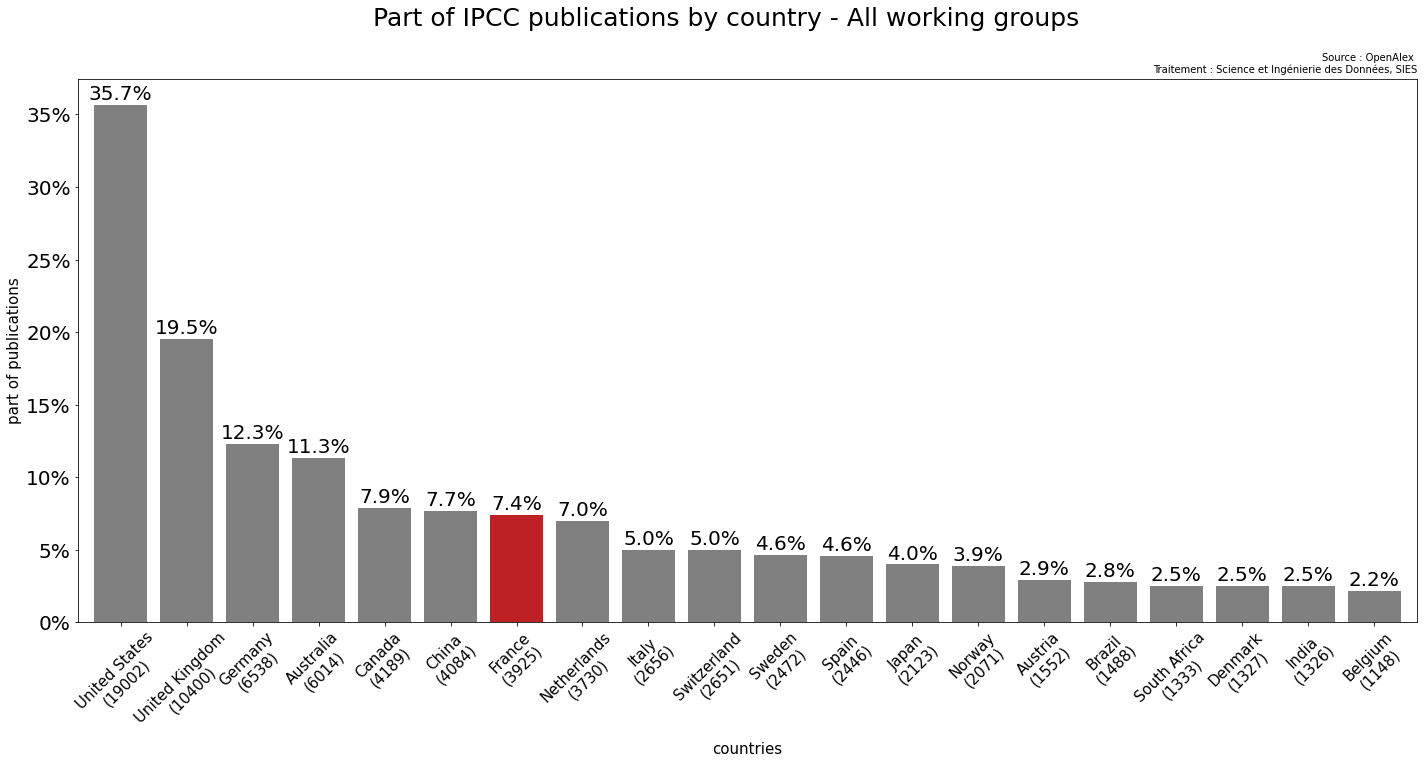
\includegraphics{./images/teds_ipcc_country_wg122cross3_part.png}
\emph{Part of IPCC publications by country for all working groups.}

In the IPBES reports, 458 French publications are cited out of a total
of 6106. This represents 7.5\% of the total publications cited. France
holds the 7th position as well in the ranking, just behind Germany and
Netherlands.

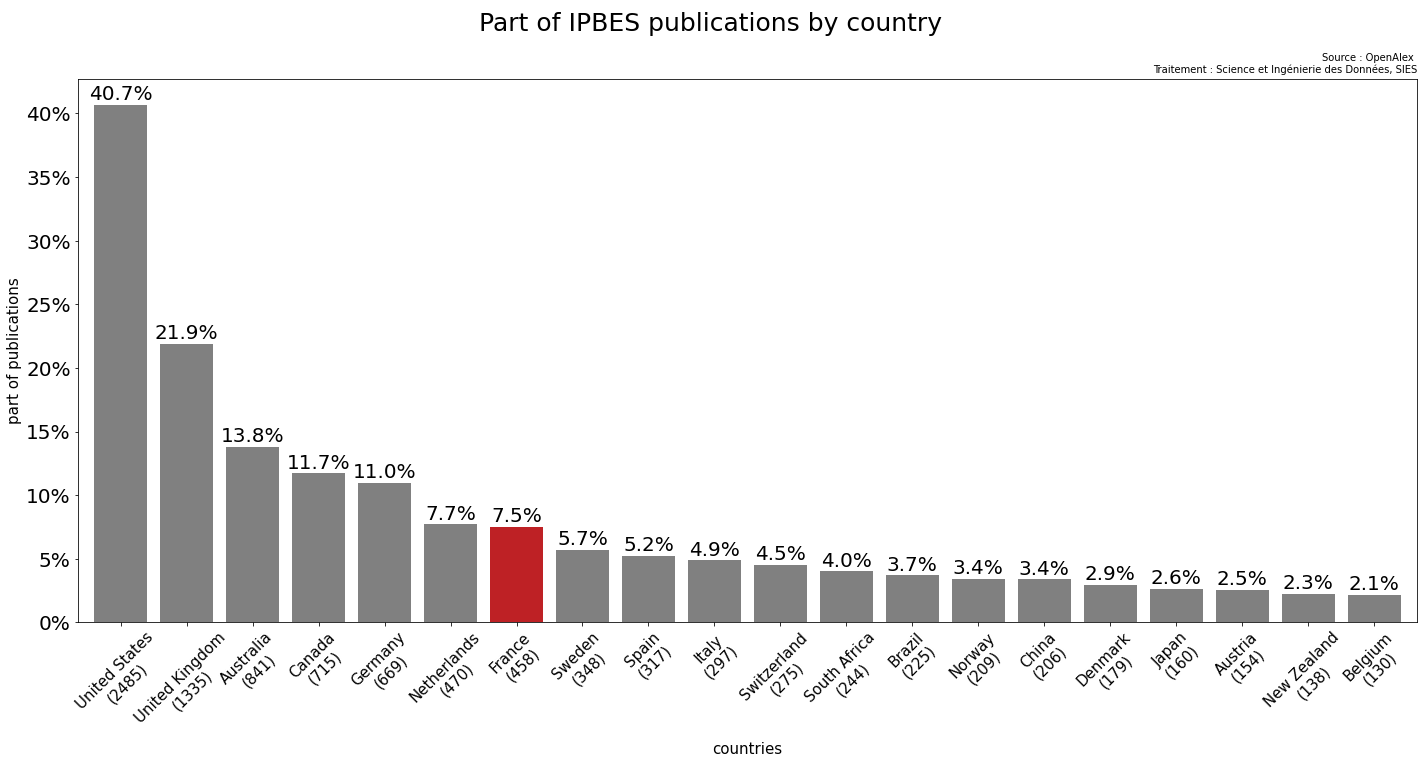
\includegraphics{./images/teds_ipbes_country_wg122cross3_part.png}
\emph{Part of IPBES publications by country.}

\hypertarget{frances-position-in-specific-research-areas}{%
\subsubsection{France's position in specific research
areas}\label{frances-position-in-specific-research-areas}}

France leads in publications related to physical sciences but is less
frequently cited in areas concerning adaptation and mitigation.

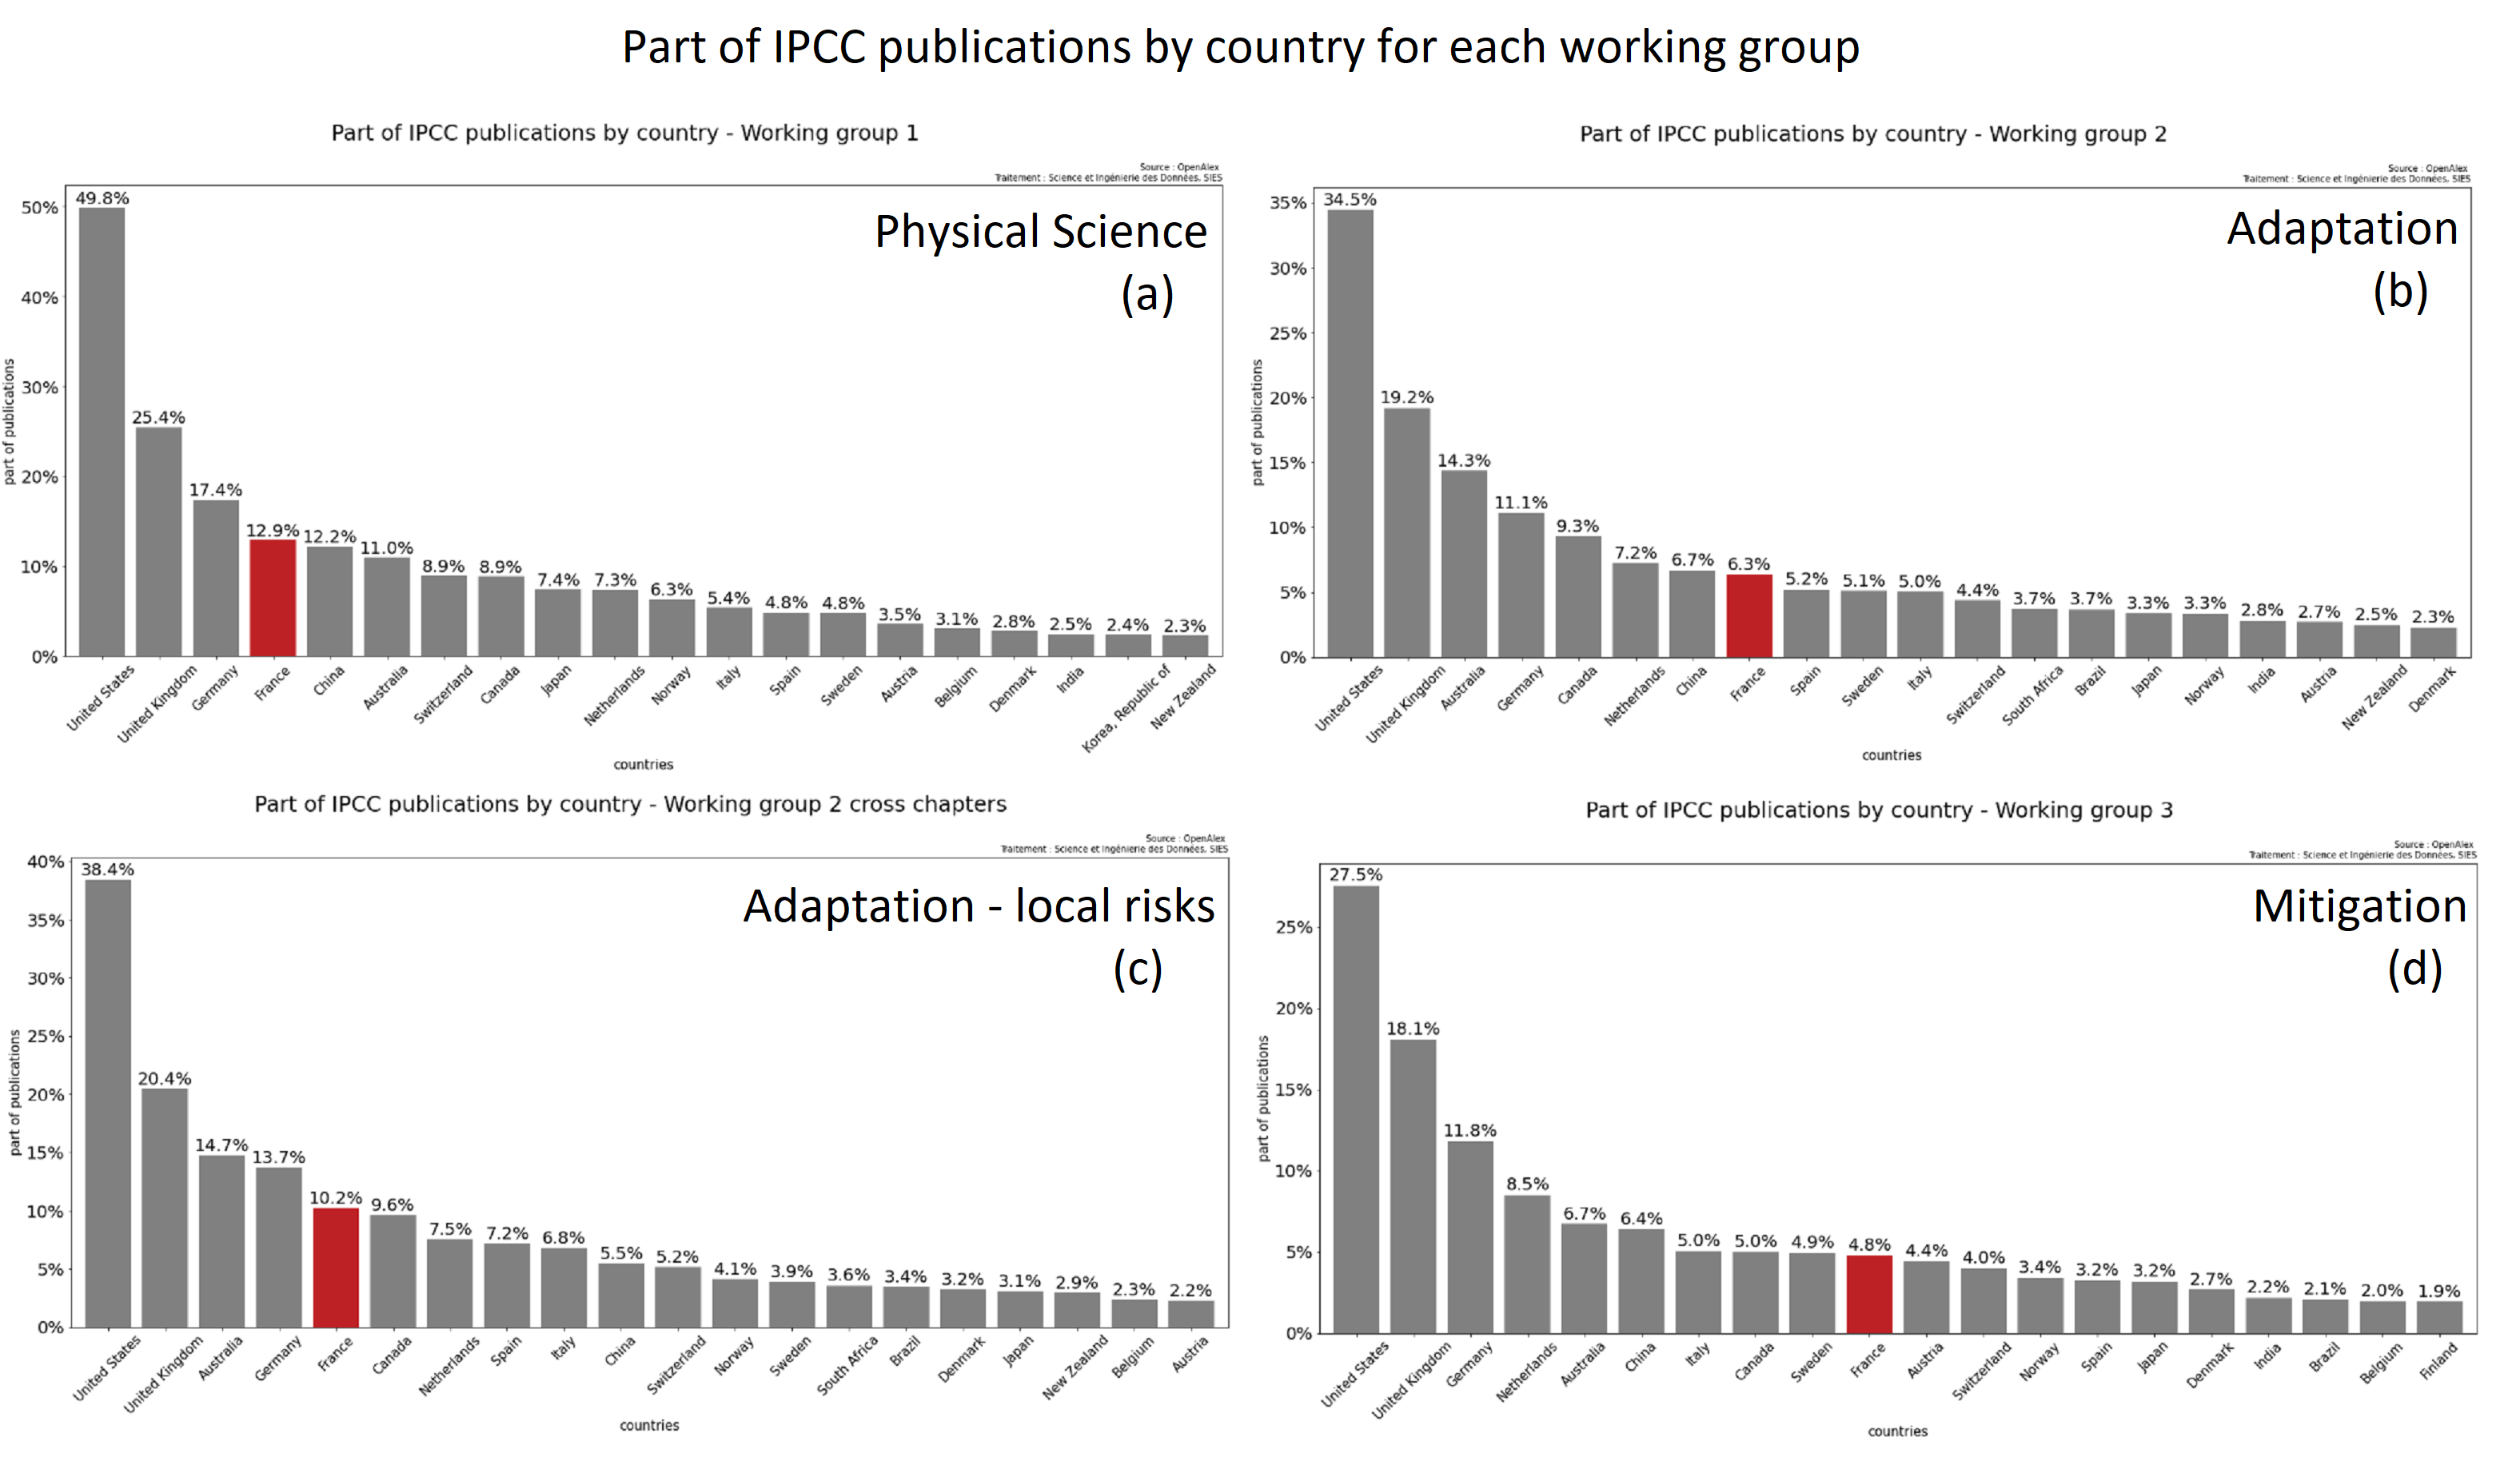
\includegraphics{./images/teds_ipcc_wg_ens_part.png} \emph{Part of IPCC
publications for each working groups.}

French publications are more concentrated than those from other
countries on theoretical sciences (a): nearly 13\% of the publications
in WG1 have a French contribution. As well as on documenting the impacts
and risks related to ecosystems such as coral reefs, forests, and
deserts (cross chapters from the second working group, the (c) image in
\emph{Part of IPCC publications for each working groups}).

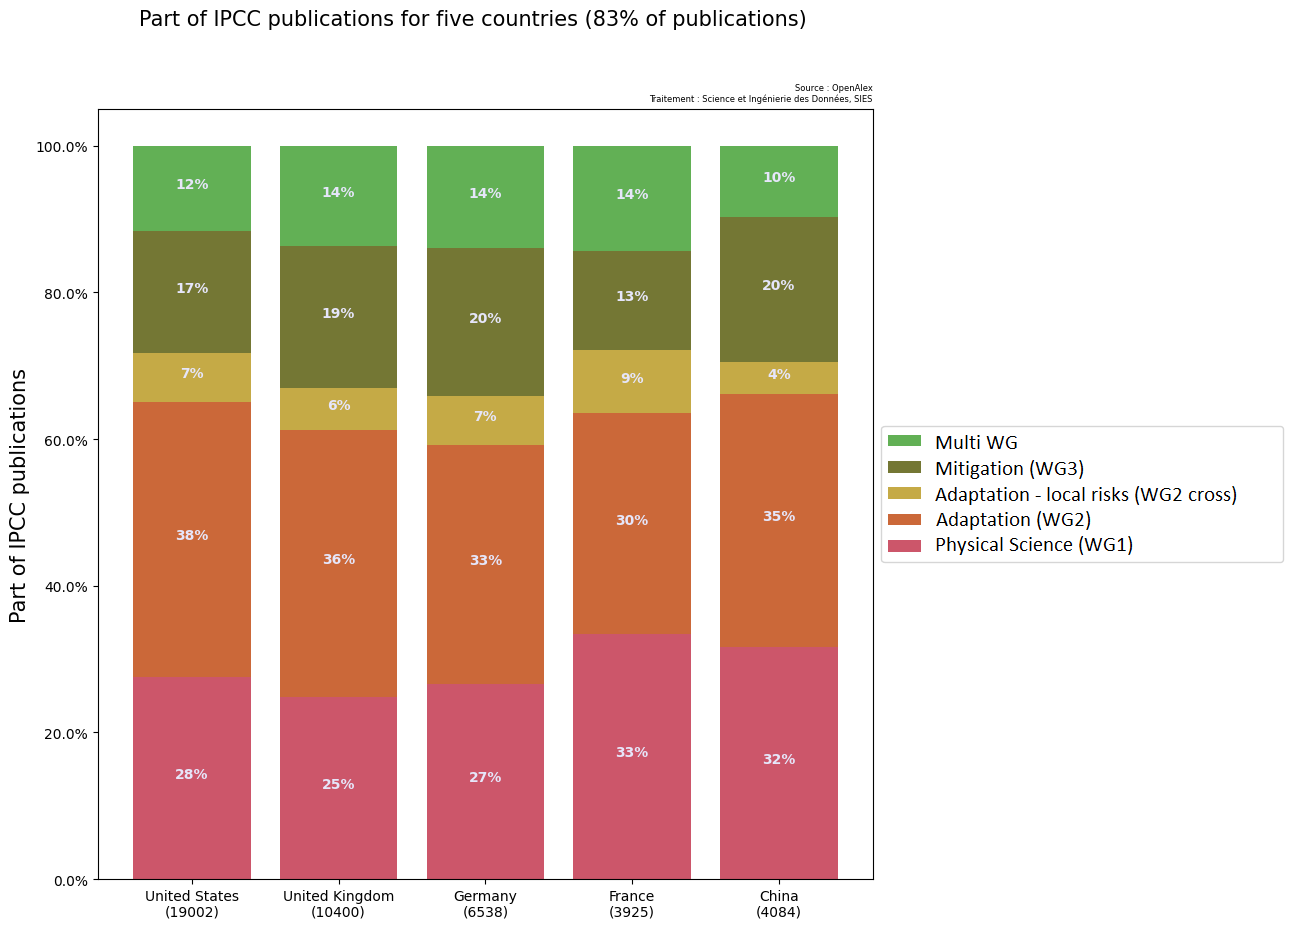
\includegraphics{./images/teds_ipcc_5countries_interfaces.png}
\emph{Part of IPCC publications for five countries.}

These findings also match those from the French Court of Audit, which
shows a strong focus on physical sciences, with less attention to
adaptation and mitigation strategies, compared to other leading
countries. Also, France, Germany, and the UK have 14\% of their
publications cited in several working groups, which is lower than the US
or China.

\hypertarget{top-institutions-laboratories-and-researchers-in-france}{%
\subsubsection{Top Institutions, Laboratories, and Researchers in
France}\label{top-institutions-laboratories-and-researchers-in-france}}

In France, the \textbf{CNRS (National Centre for Scientific Research)}
is a leader in IPCC and IPBES publications, with IRD (Research Institute
for Development) also making significant contributions.

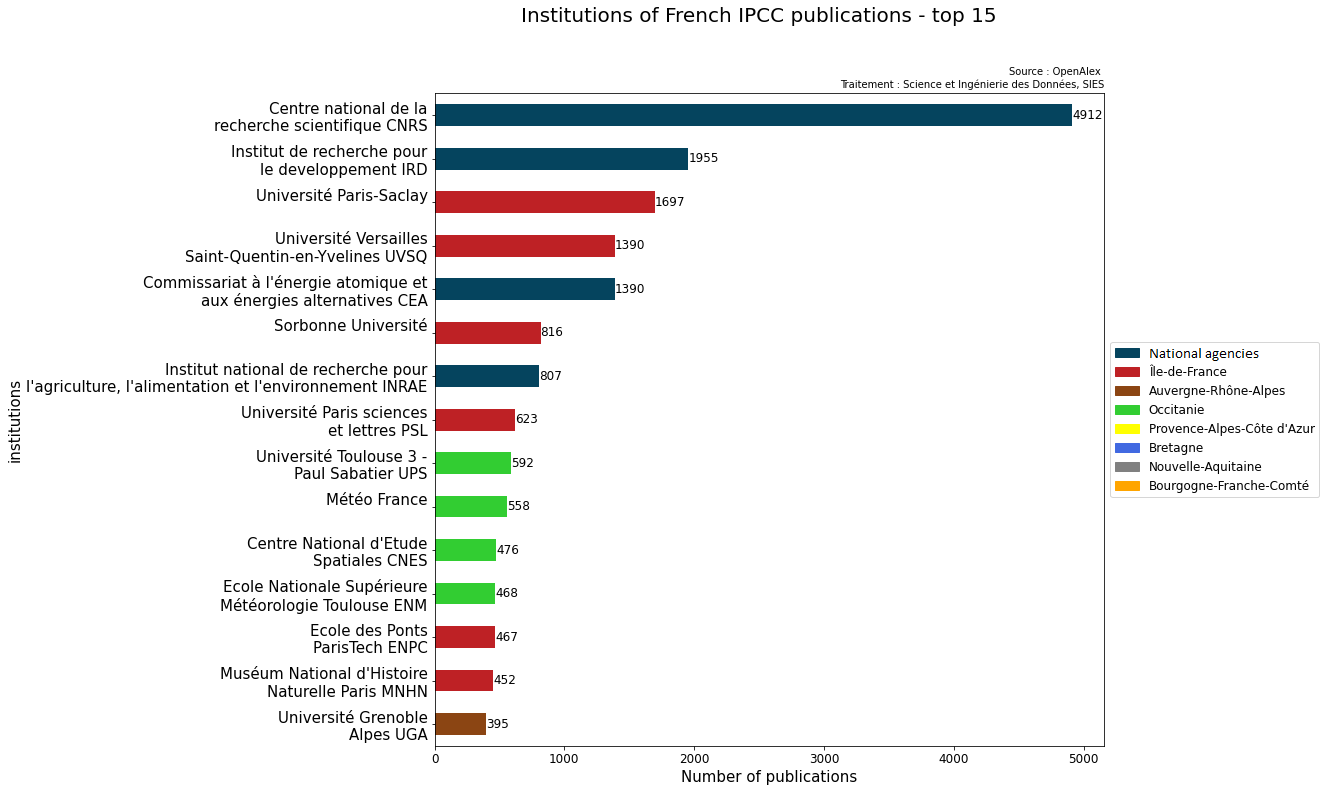
\includegraphics{./images/teds_ipcc_institutions.png} \emph{French
institutions contributing to IPCC publications.}

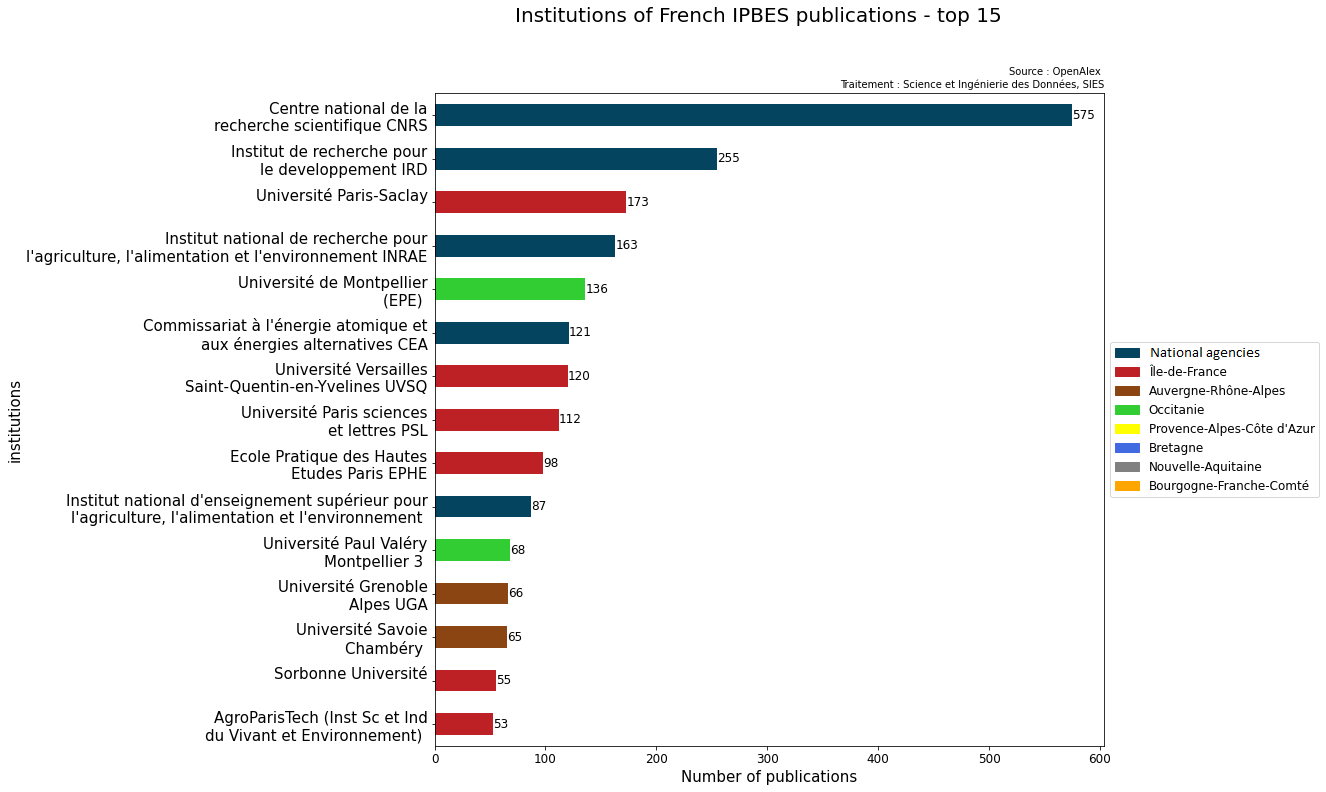
\includegraphics{./images/teds_ipbes_institutions.png} \emph{French
institutions contributing to IPBES publications.}

We can see that several national organizations appear in both reports,
however there is a clear territorial difference at the institutional
level. The institutions most active in the IPCC publications are mainly
located in Île-de-France, Toulouse, and Grenoble, while those in the
IPBES publications are mostly in Île-de-France, Grenoble, Chambéry, and
Montpellier.

The \textbf{Climate Science Laboratory} is another key player in climate
research, leading the way in IPCC and IPBES publications.

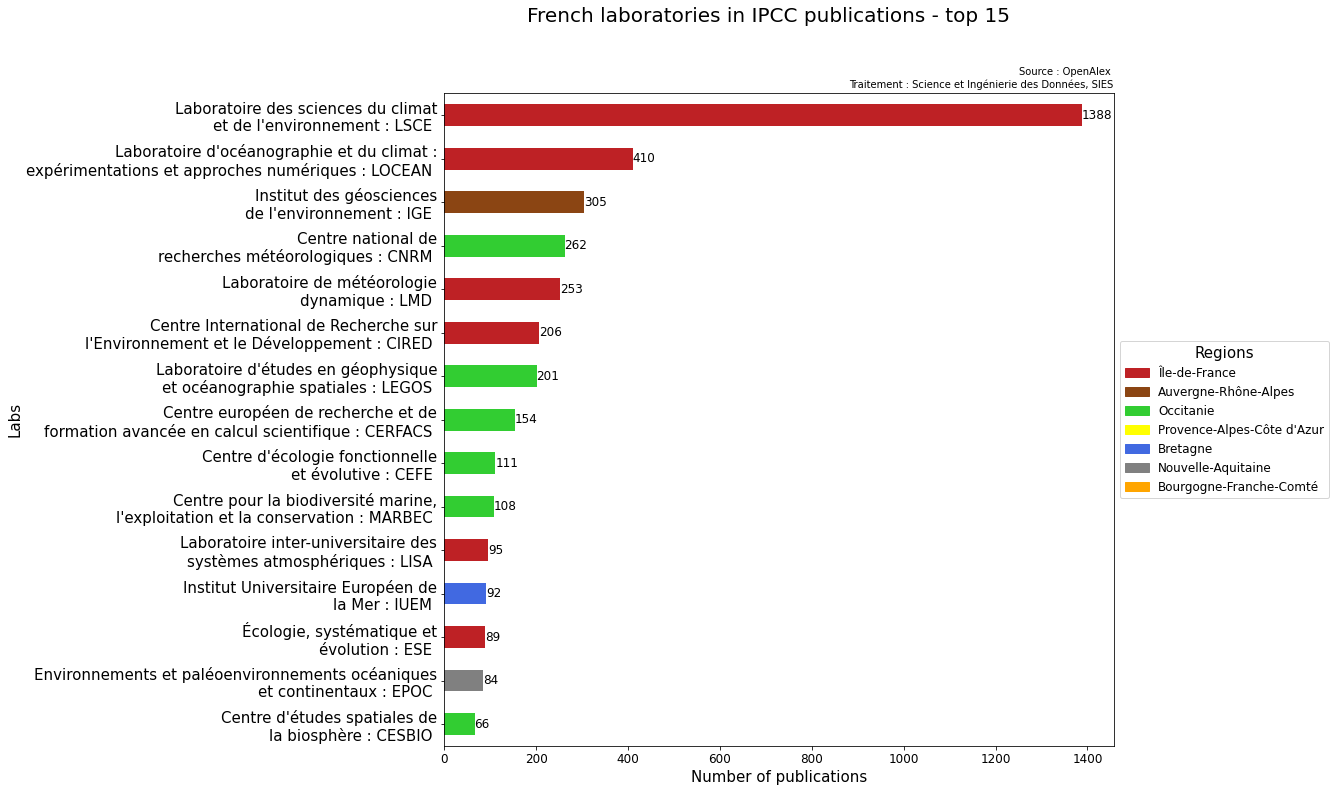
\includegraphics{./images/teds_ipcc_lab.png} \emph{French laboratories
contributing to IPCC publications.}

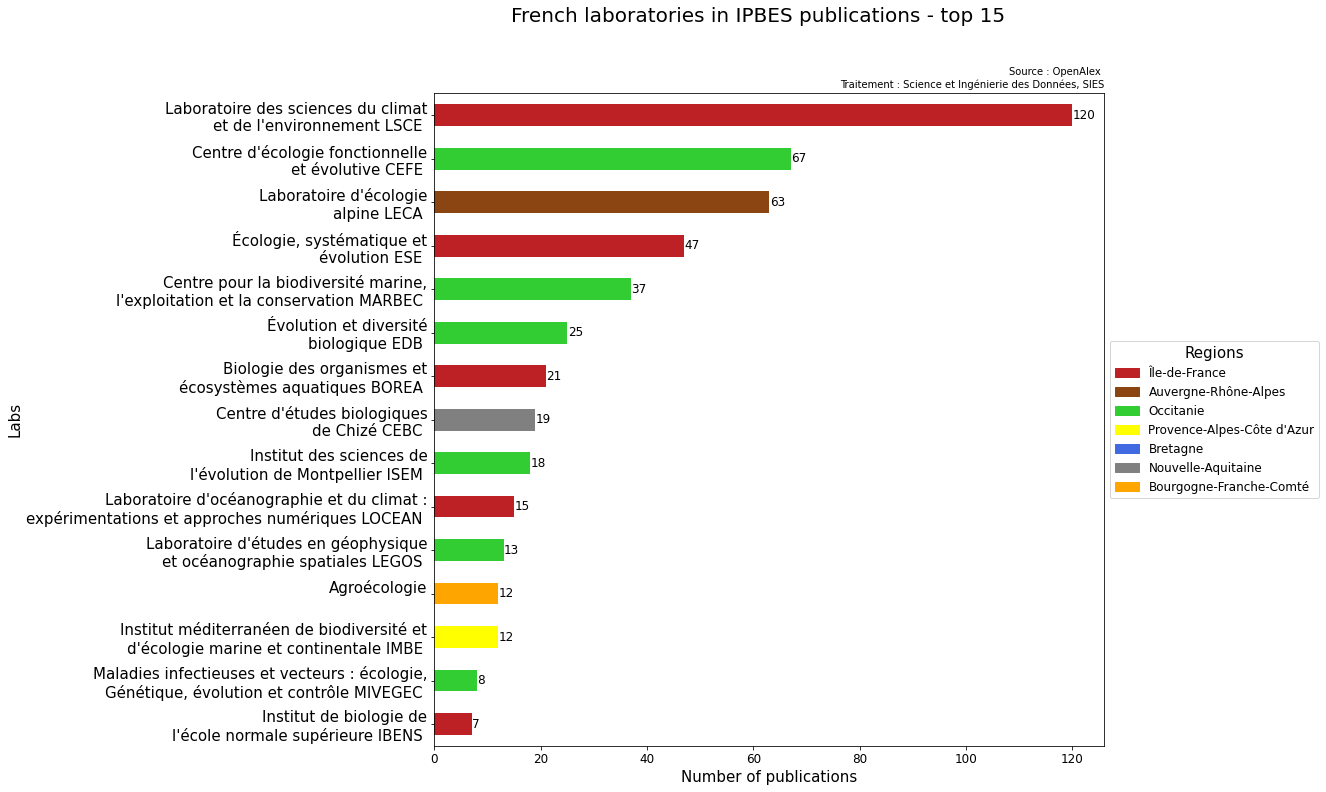
\includegraphics{./images/teds_ipbes_labs.png} \emph{French laboratories
contributing to IPBES publications.}

The laboratories most active in the publications cited by the IPCC are
located mainly in Île-de-France, Toulouse, Grenoble, Bretagne and
Bordeaux. Those of the IPBES are located in Île-de-France, Montpellier,
Grenoble, Toulouse, Chizé, Dijon and Marseille.

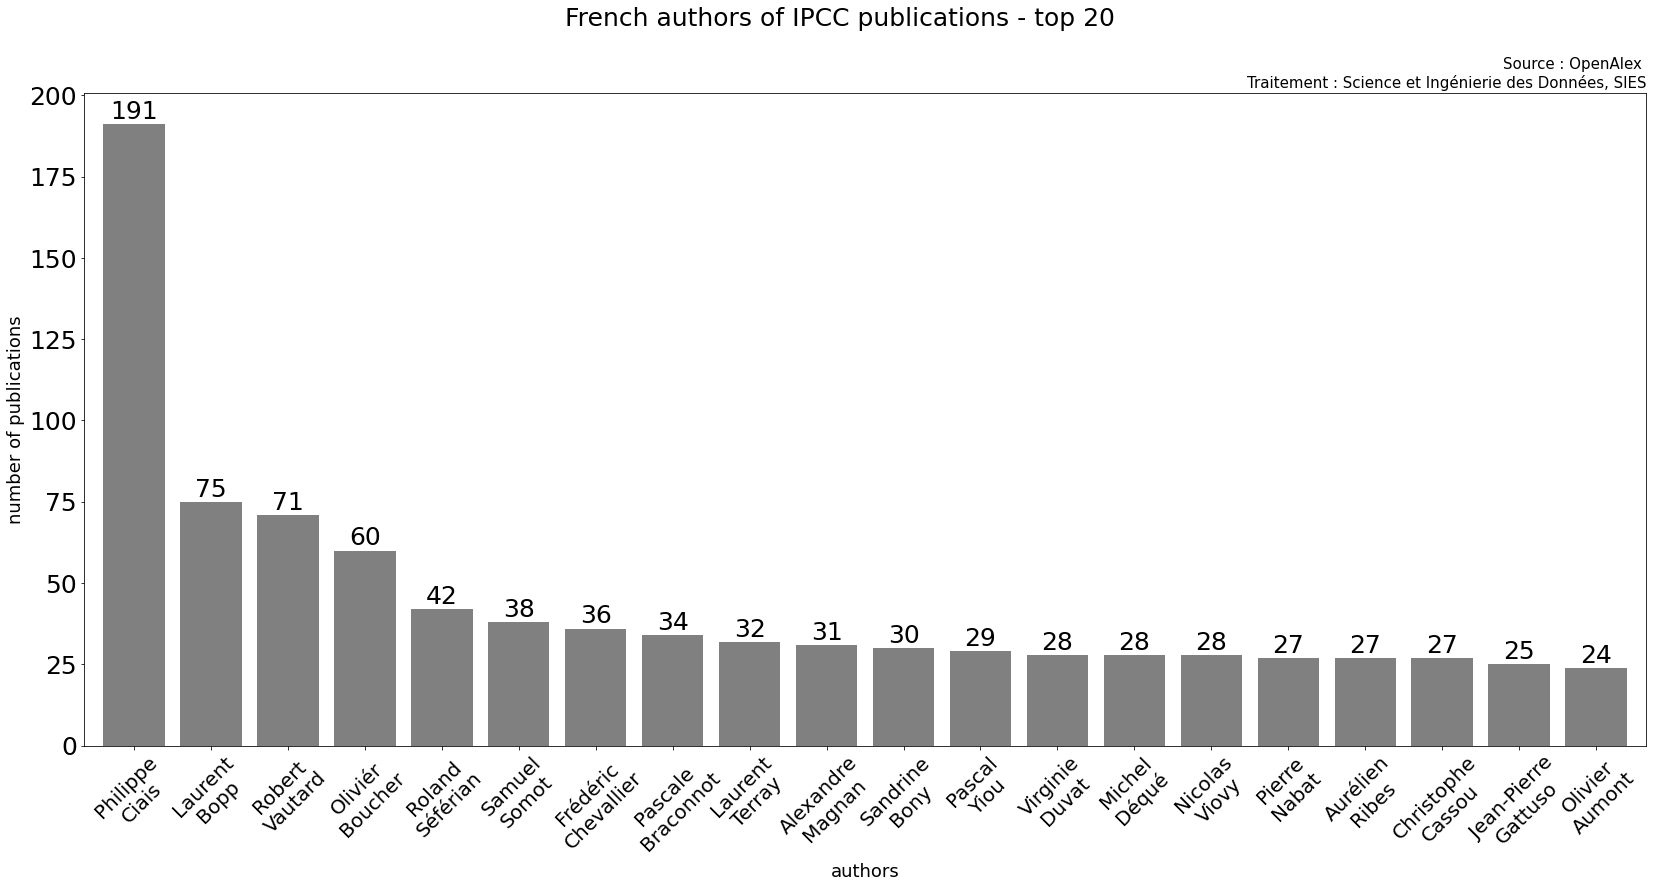
\includegraphics{./images/teds_ipcc_authors.png} \emph{French authors
contributing to IPCC publications.}

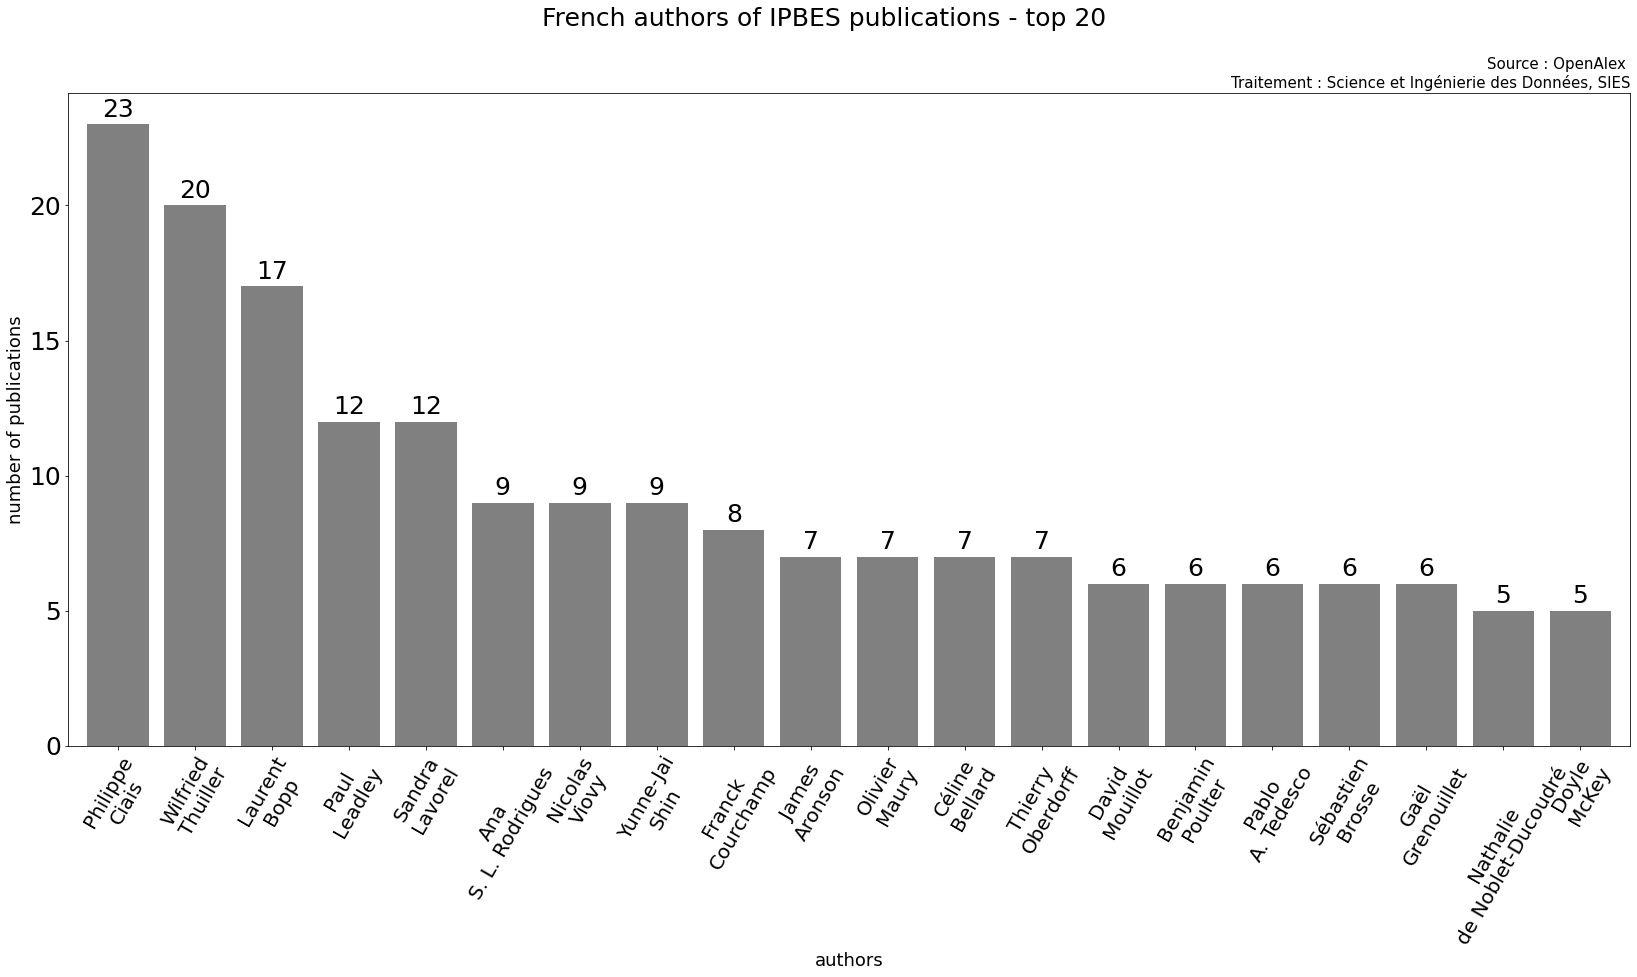
\includegraphics{./images/teds_ipbes_authors.png} \emph{French authors
contributing to IPBES publications.}

French researchers are also highly involved, with some contributing to
both IPCC and IPBES reports. For example, Philippe Ciais is particularly
active and cited in both reports.

\hypertarget{models-performances} of the
total publications.

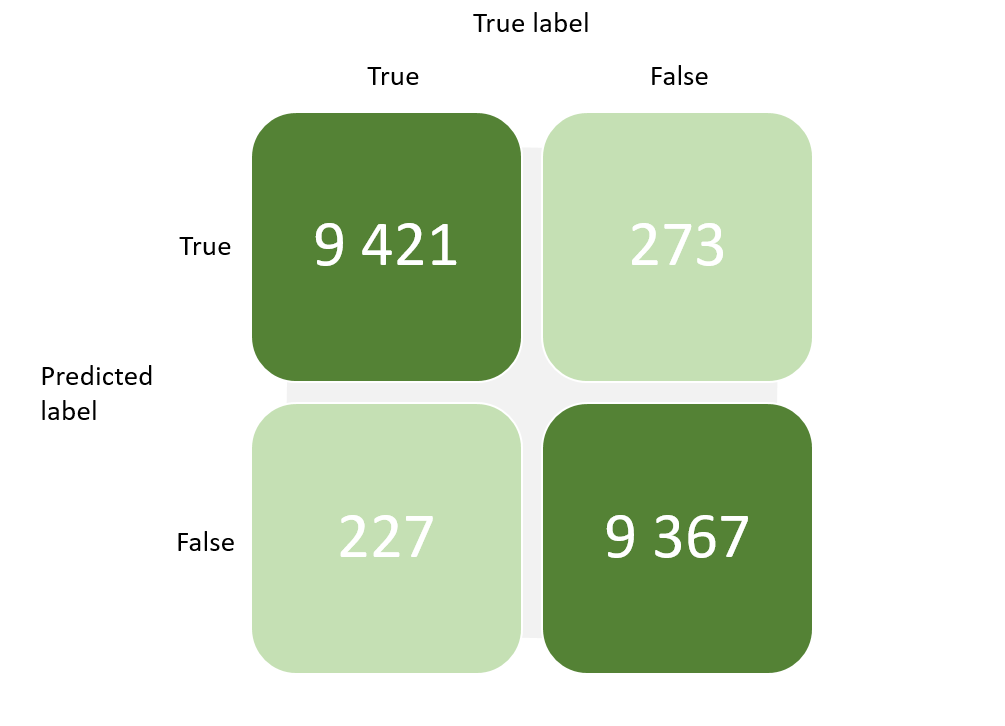
\includegraphics{./images/teds_ipcc_model.png} \emph{Confusion matrix
showing the performance of the first IPCC model.}

When a publication is identified as ``IPCC-like'', a second model is
applied to classify it into the appropriate working group. The second
model predicts which working group the publication is most likely
associated with.

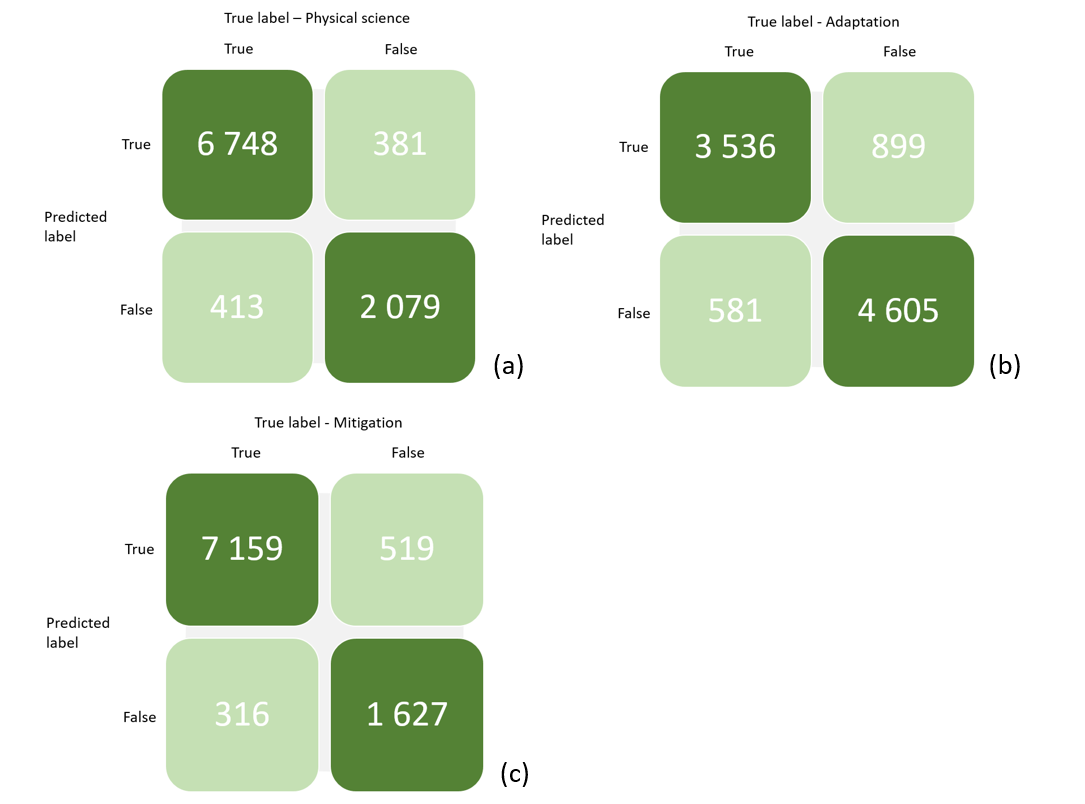
\includegraphics{./images/teds_ipcc_model_wg.png} \emph{Confusion matrix
illustrating the performance of the second IPCC model, which categorizes
publications by working group.}

For each working group, there are 9,644 publications in the test set.
The model performance for each group is as follows:

\begin{itemize}
\tightlist
\item
  For \textbf{Physical Science}, 8,875 publications are correctly
  predicted, representing \textbf{92\%} of the publications in this
  category.
\item
  For \textbf{Adaptation}, 8,137 publications are correctly predicted,
  representing \textbf{84\%} of the publications in this category.
\item
  For \textbf{Mitigation}, 8,768 publications are correctly predicted,
  representing \textbf{91\%} of the publications in this category.
\end{itemize}

However, for the \textbf{Adaptation} and \textbf{Mitigation} categories,
the model shows a significant number of false positives. This suggests
that the model tends to overestimate the number of publications
categorized in these groups. This overestimation indicates that the
model might label more publications as ``Adaptation'' or ``Mitigation''
than is strictly accurate, leading to a higher rate of false positives
in these categories.

\hypertarget{the-models-on-scanr-publications}{%
\subsection{3.3 The models on ScanR
publications}\label{the-models-on-scanr-publications}}

\hypertarget{figures}{%
\subsubsection{Figures}\label{figures}}

\texttt{invistiguer\ les\ publis\ ipcc\ qui\ ont\ disparues:\ 70k\ =\textgreater{}\ 52k}
We focus on references with a DOI in scanR, as my analysis depends on
these type of work, excluding other type such as theses, which follow a
different structure. This ensure consistency in our resonnement. The
proportion of publications addressing topics similar to those of the
IPCC seems to be increasing in recent years. The graph ``IPCC model on
scanR publications by year'' illustrates this trend, showing a growing
number of ``IPCC-like'' publications in scanR over time.

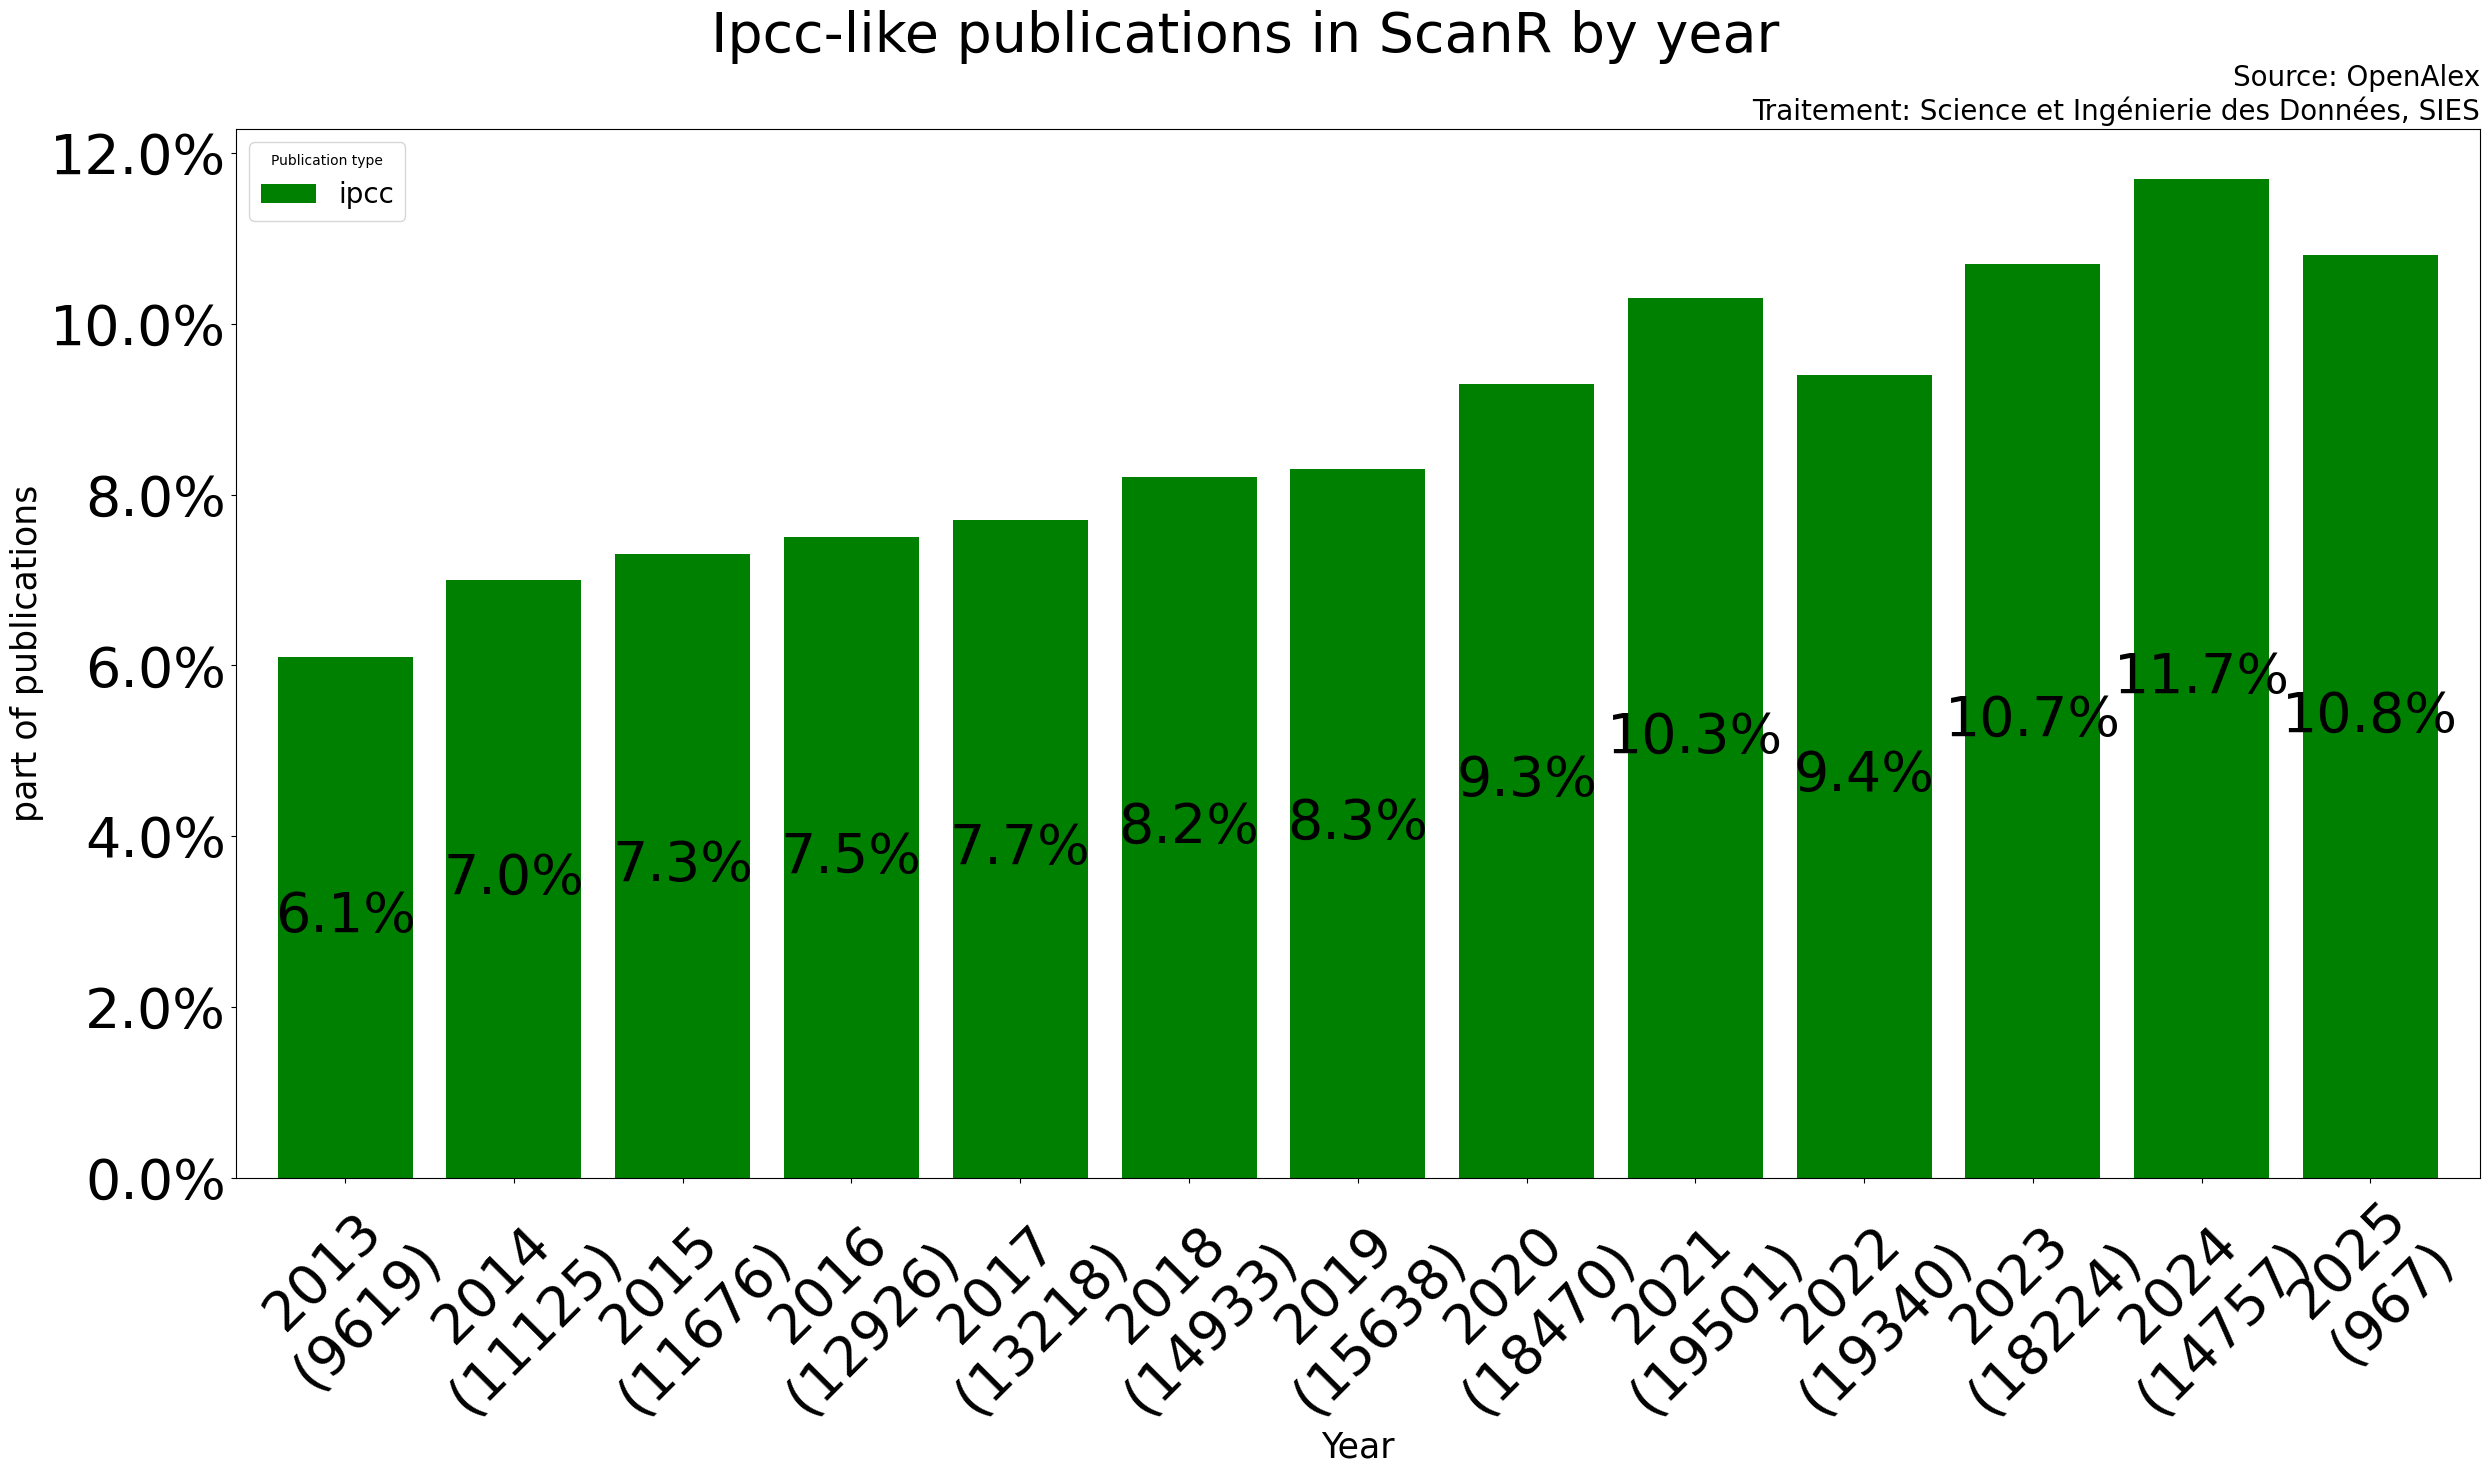
\includegraphics{./images/teds_model_scanR1.png} \emph{IPCC model on
scanR publications by year.}

The second model seems to detect more publications related to
adaptation.

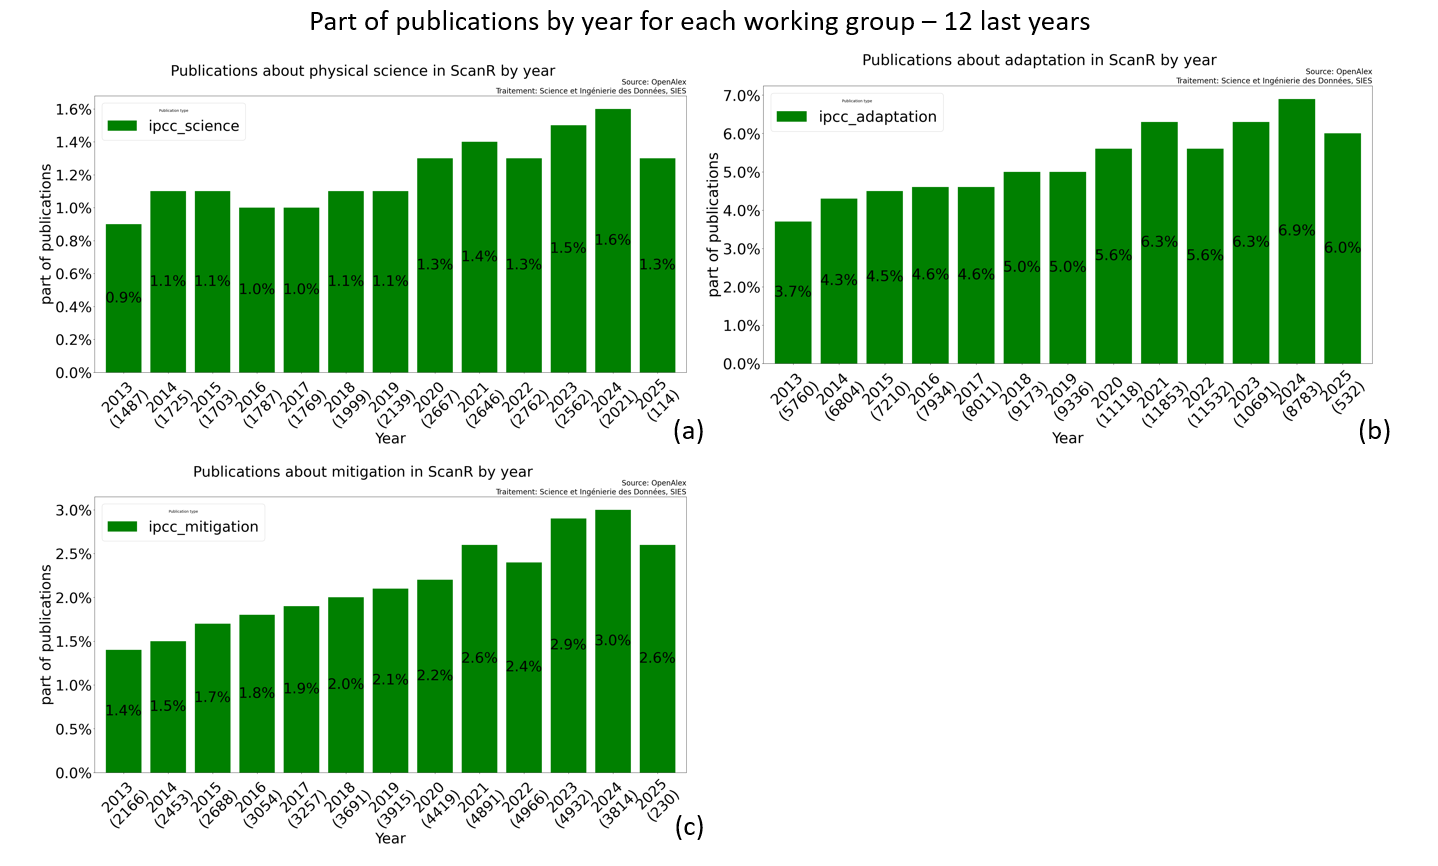
\includegraphics{./images/teds_model_scanR_wg.png} \emph{Working group
model on scanR publications by year.}

\hypertarget{community-network}{%
\subsubsection{Community network}\label{community-network}}

On scanR, we can visualize community network, based on themes or on
authors.

A community network is a way to group things together based on how
closely they are connected. In this case, a ``node'' is either an author
or a theme, and a ``link'' is a co-publication between them. It's like
finding clusters of authors or themes that are more connected to each
other through co-publications than to others outside the group. These
groups, called communities, help us understand how the system is
organized and how different parts work together. Looking at these groups
can help us find patterns and learn more about the connections between
authors or themes(Barbier 2025).

The topics cited by the IPCC cover a broad range of topics, and the
IPCC's publication network is denser than that predicted by the model.
This indicates that the topics are often cited together across multiple
publications. The graph \emph{Comparaison between two topics networks.}
shows two topic networks: one showing the denser network from IPCC
reports (a) and the other representing the less interconnected predicted
network from the first model (b). From this, we can conclude that the
topics in the IPCC reports are more tightly interconnected.
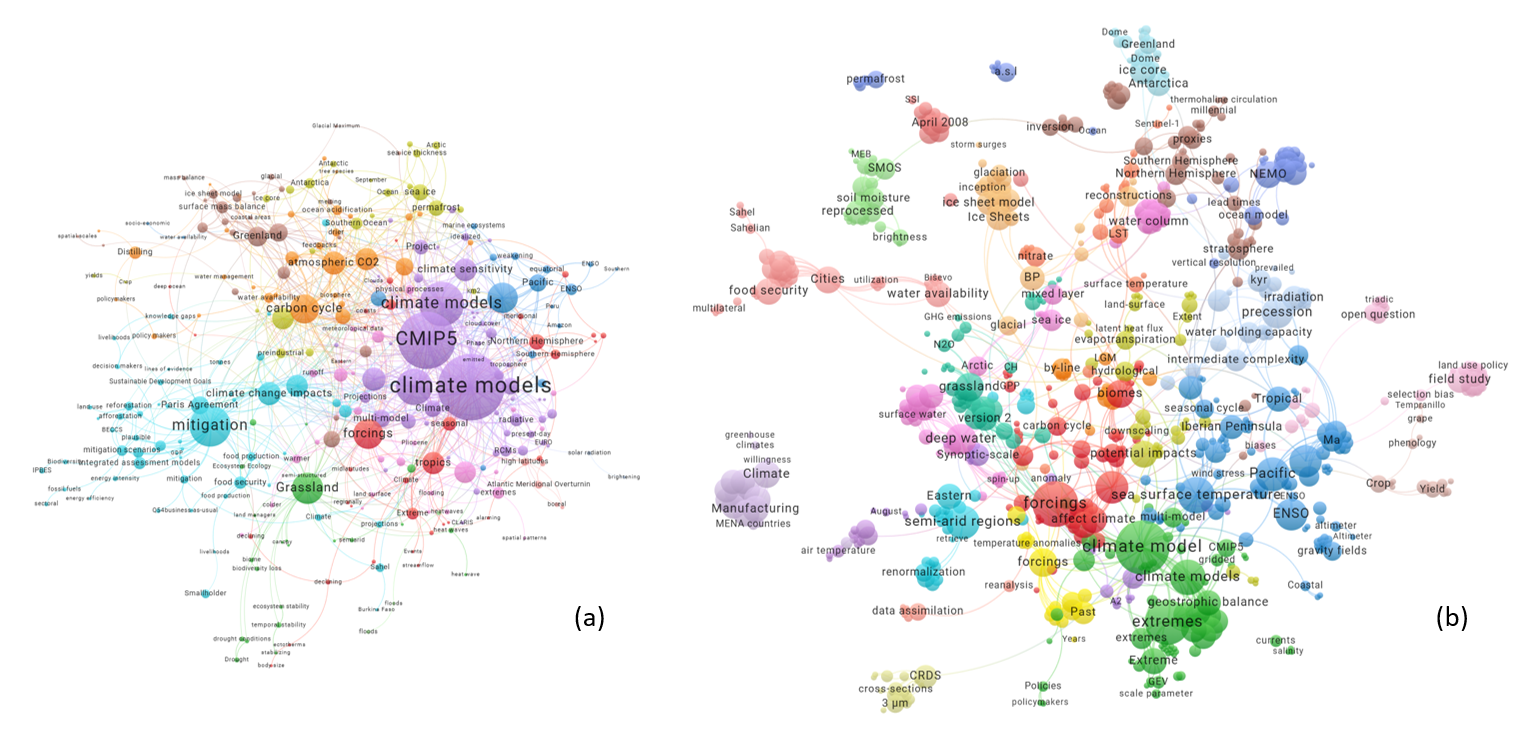
\includegraphics{./images/teds_network_topics2.png} \emph{Comparaison
between two topics networks.}

It's interesting to see that `soil moisture' is linked to
`evapotranspiration' in both graphs, but the predicted graph (d)
introduces more technical terms. In this graph, `soil moisture' is
connected to `SMOS' and `L-band.' SMOS is a satellite from the European
Space Agency (ESA) that measures soil moisture using radiation in the
L-band (1.4 GHz). This shows that the predicted graph can focuses on
more technical details.
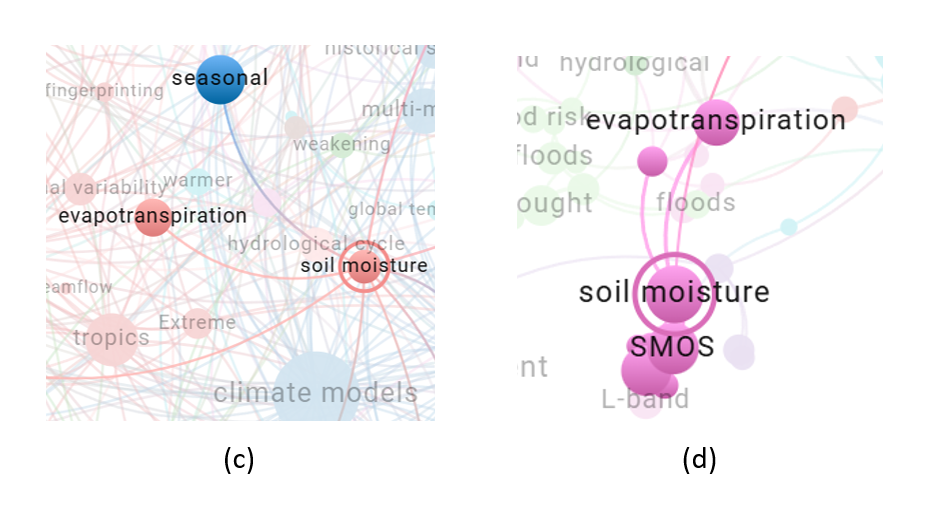
\includegraphics{./images/teds_network_topics2_sensors.png}
\emph{Comparaison on one topic.}

We can see a similar dynamic for authors, a denser network for authors
from IPCC reports (e). we can see a principal block composed by Philippe
Ciais and Laurent Bopp that represent an ``IPCC cluster''\\
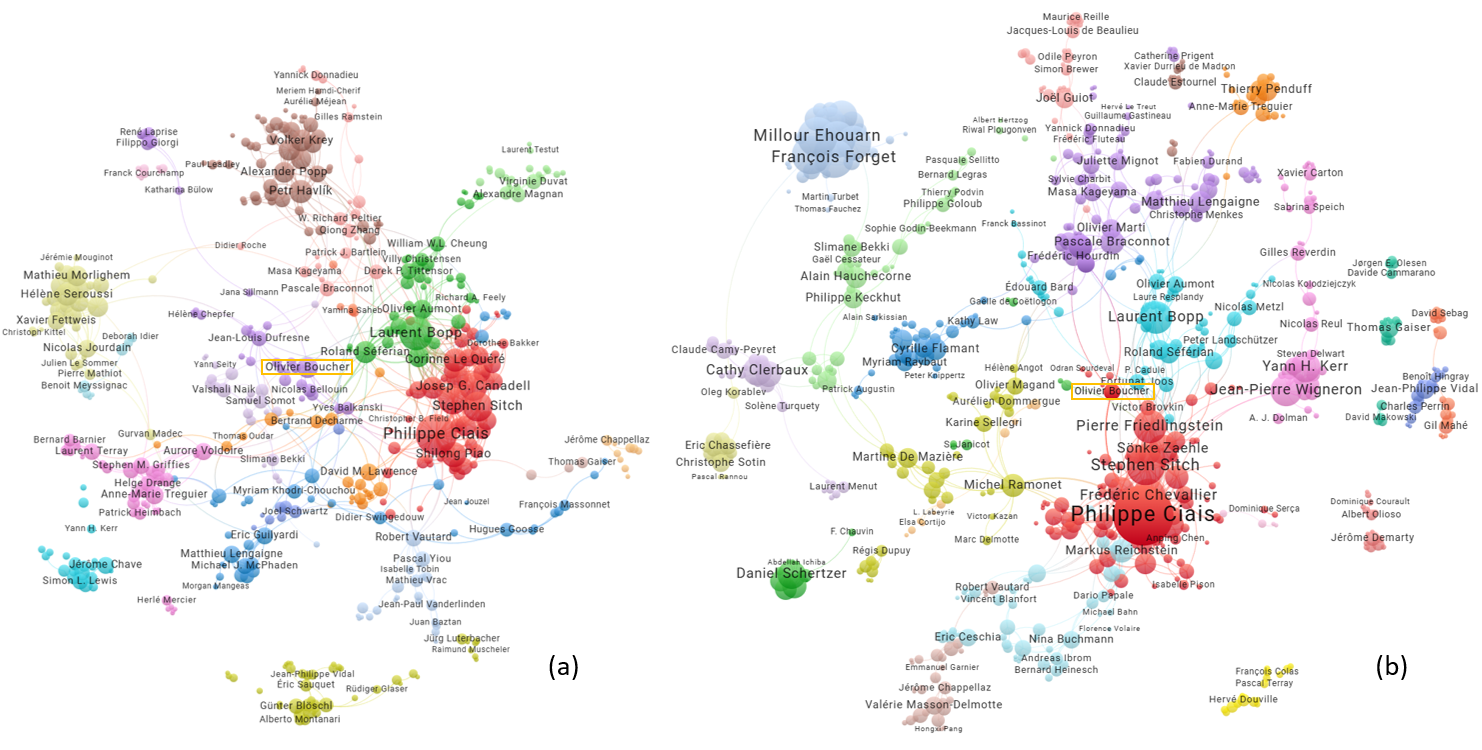
\includegraphics{./images/teds_network_authors2.png} \emph{Comparaison
between two authors networks.}

\hypertarget{on-openalex}{%
\subsection{3.4 On OpenAlex}\label{on-openalex}}

\includegraphics{./images/teds_OA_part10.png} \emph{Part of publications
in OpenAlex for 10 countries.}

\includegraphics{./images/teds_OA_rank10.png} \emph{Rank for 10
countries in OpenAlex publications.}

\hypertarget{code-availibility}{%
\section{4. Code availibility}\label{code-availibility}}

The code developed is open source and available online on GitHub
\url{https://github.com/dataesr/teds}

\hypertarget{references}{%
\section{References}\label{references}}

\begin{verbatim}
\end{verbatim}

\hypertarget{refs}{}
\begin{cslreferences}
\leavevmode\hypertarget{ref-hal-04892262}{}%
Barbier, Jeangirard. 2025. ``Mapping Scientific Communities at Scale,''
no. 1 (January). \url{https://hal.science/hal-04892262v1}.

\leavevmode\hypertarget{ref-10.1162ux2fqss_a_00179}{}%
Chaignon, Lauranne, and Daniel Egret. 2022. ``Identifying Scientific
Publications Countrywide and Measuring Their Open Access: The Case of
the French Open Science Barometer (Bso).'' \emph{Quantitative Science
Studies} 3 (1): 18--36. \url{https://doi.org/10.1162/qss_a_00179}.

\leavevmode\hypertarget{ref-ipccbibliography}{}%
n.d.a. \url{https://www.ipcc.ch/report/ar6}.

\leavevmode\hypertarget{ref-ipbesbibliography}{}%
n.d.b.
\url{https://www.zotero.org/groups/2333077/ipbes_global_assessment/library}.
\end{cslreferences}


\end{document}
